%!TEX program = xelatex
\documentclass[fontset=none, a4paper, 12pt]{ctexart}

% ==========================================
% 1. 套件載入區（國立中興大學制式模板規範）
% ==========================================
\usepackage{geometry}
\usepackage{longtable}
\usepackage{fontspec}
\usepackage{setspace}
\usepackage{titlesec}
\usepackage{titletoc}
\usepackage{tocloft}
\usepackage{fancyhdr}
\usepackage{graphicx}
\usepackage{caption}
\captionsetup[figure]{skip=4pt}
\captionsetup[table]{skip=4pt}
\setlength{\intextsep}{8pt}
\setlength{\textfloatsep}{8pt}
\setlength{\floatsep}{8pt}
\usepackage[hidelinks]{hyperref}
\usepackage{booktabs}
\usepackage{float}
\usepackage{amsmath}
\usepackage{amssymb}
\usepackage{tabularx}
\usepackage{placeins}
\usepackage{needspace}
\usepackage{algorithm}
\usepackage{algpseudocode}
\floatname{algorithm}{演算法}
\usepackage{makecell}
\usepackage{array}
\usepackage{pdflscape}
\usepackage{rotating}
\usepackage{pdfpages}
\sloppy

% ==========================================
% 2. 字型設定（自帶 TTF 確保跨平台與 Overleaf 100% 一致）
% ==========================================
\setCJKmainfont{kaiu.ttf}[
    AutoFakeBold=2.5,
    AutoFakeSlant=0.3
]
\setmainfont{LiberationSerif-Regular.ttf}[
    BoldFont=LiberationSerif-Bold.ttf,
    ItalicFont=LiberationSerif-Italic.ttf,
    BoldItalicFont=LiberationSerif-BoldItalic.ttf
]
\newCJKfontfamily\coverzh{kaiu.ttf}[
    AutoFakeBold=2.5,
    AutoFakeSlant=0.3
]
\newfontfamily\coveren{LiberationSerif-Regular.ttf}[
    BoldFont=LiberationSerif-Bold.ttf,
    ItalicFont=LiberationSerif-Italic.ttf,
    BoldItalicFont=LiberationSerif-BoldItalic.ttf
]

% ==========================================
% 3. 版面與格式設定
% ==========================================
\geometry{a4paper, top=3cm, bottom=3cm, left=3cm, right=3cm}
\pagestyle{plain}

% 圖表標題中文化
\captionsetup[figure]{name=圖}
\captionsetup[table]{name=表}
\ctexset{bibname = {參考文獻}}

% 章節標題格式
\titleformat{\section}[block]{\centering\fontsize{20}{24}\selectfont\bfseries}{\thesection}{1em}{}
\titleformat{\subsection}[block]{\fontsize{16}{20}\selectfont\bfseries}{\thesubsection.}{1em}{}
\titleformat{\subsubsection}[block]{\fontsize{14}{18}\selectfont\bfseries}{\thesubsubsection.}{1em}{}

% 編號格式
\renewcommand{\thesection}{第\chinese{section}章}
\renewcommand{\thesubsection}{\arabic{section}.\arabic{subsection}}
\renewcommand{\thesubsubsection}{\arabic{section}.\arabic{subsection}.\arabic{subsubsection}}

% 目錄、表目錄、圖目錄設定
\renewcommand{\contentsname}{目錄}
\renewcommand{\listtablename}{表目錄}
\renewcommand{\listfigurename}{圖目錄}

\renewcommand{\cfttoctitlefont}{\hfill\Large\bfseries}
\renewcommand{\cftaftertoctitle}{\hfill\null}
\renewcommand{\cftlottitlefont}{\hfill\Large\bfseries}
\renewcommand{\cftafterlottitle}{\hfill\null}
\renewcommand{\cftloftitlefont}{\hfill\Large\bfseries}
\renewcommand{\cftafterloftitle}{\hfill\null}

\setlength{\cftbeforetoctitleskip}{0pt}
\setlength{\cftaftertoctitleskip}{0.8em}
\setlength{\cftbeforelottitleskip}{0pt}
\setlength{\cftafterlottitleskip}{1.0em}
\setlength{\cftbeforeloftitleskip}{0pt}
\setlength{\cftafterloftitleskip}{1.0em}

\renewcommand{\cftsecleader}{\cftdotfill{\cftdotsep}}
\renewcommand{\cftsubsecleader}{\cftdotfill{\cftdotsep}}
\renewcommand{\cftsubsubsecleader}{\cftdotfill{\cftdotsep}}

\renewcommand{\cftsecfont}{\bfseries}
\renewcommand{\cftsecpagefont}{\bfseries}
\setlength{\cftbeforesecskip}{0.35em}

\begin{document}

% ==========================================
% 封面（依學校制式範本與指定文字精確排版）
% ==========================================
\newgeometry{a4paper, top=3cm, bottom=3cm, left=3cm, right=3cm}
\begin{titlepage}
    \centering
    \thispagestyle{empty}
    \vspace*{0.7cm}

    {\coverzh
    \fontsize{20pt}{28pt}\selectfont
    \begingroup
    \xeCJKsetup{CJKglue=\hskip -1.55pt}
    \makebox[\textwidth][c]{國立中興大學人工智慧與資料科學碩士在職學位學程}
    \endgroup
    \par}

    \vspace{0.35cm}
    {\coverzh\fontsize{20pt}{28pt}\selectfont 碩士學位論文\par}

    \vspace{2.4cm}
    {\coverzh\fontsize{20pt}{29pt}\selectfont
    半導體製程冷卻水系統時間序列監測的\\異常檢測與預警\par}

    \vspace{0.75cm}
    {\coveren\fontsize{18pt}{24pt}\selectfont
    \makebox[\textwidth][c]{Anomaly Detection and Early Warning for Time-Series Monitoring}%
    \par
    \makebox[\textwidth][c]{of Semiconductor Process Cooling Water Systems}%
    \par}

    \vspace{2.4cm}
    {\coverzh\fontsize{20pt}{28pt}\selectfont
    指導教授：\hspace{0.3em}吳宏達\par}

    \vspace{0.35cm}
    {\coverzh\fontsize{20pt}{28pt}\selectfont
    研究生：\hspace{0.3em}陳 宥興\par}

    \vspace{2.0cm}
    {\coverzh\fontsize{20pt}{28pt}\selectfont 中華民國一百一十五 年十一月\par}
\end{titlepage}
\restoregeometry
\clearpage

% ==========================================
% 口試審核頁預留（依模板預留空白頁）
% ==========================================
\thispagestyle{empty}
\vspace*{\fill}
\begin{center}
    \Large 口試審核頁預留
\end{center}
\vspace*{\fill}
\clearpage

% ==========================================
% 誌謝（不顯示頁碼，目錄不列入）
% ==========================================
\clearpage
\pagenumbering{gobble}
\pagestyle{empty}
\begin{center}
    \large\bfseries 誌謝
\end{center}
\vspace{0.5em}

碩士研究歷程的完成，首先由衷感謝指導教授吳宏達博士在人工智慧、統計品質管制與工業物聯網架構領域的悉心指導與鞭策。老師嚴謹的治學態度、對理論公式與實體工程落地並重之堅持，奠定了本論文兼具學術深度與工業實用性的基石。

特別感謝產業界先進與實驗室同儕在工業通訊協定、Modbus/TCP 暫存器架構與微秒級時序推論驗證過程中的寶貴交流。感謝家人的無條件支持與體諒，使我得以在長程全廠 3,840 場自動化測試、演算法硬化調校與全端 SCADA 開發過程中保持專注，終能順利完成學位論文。謹將本研究成果獻給所有支持與關心我的師長、家人與摯友。

\vspace{2em}
\begin{flushright}
陳 宥興　謹誌\\
中華民國一百一十五年十一月
\end{flushright}

% ==========================================
% 前半部：羅馬數字頁碼 (i, ii, iii...)
% ==========================================
\clearpage
\pagestyle{plain}
\pagenumbering{roman}
\setcounter{page}{1}

\phantomsection
\addcontentsline{toc}{section}{摘要}
\begin{center}
\large\bfseries 摘要
\end{center}
\vspace{0.5em}

製程冷卻水（Process Cooling Water, PCW）為半導體先進製程晶圓廠維持微影、蝕刻與化學沉積等關鍵設備熱平衡之核心公用系統。現行工業 SCADA 多採靜態固定門檻（HI/HIHI/LO/LOLO）觸發警報，雖具規則明確優勢，但警報發出時壓力數值往往已突破安全邊界，操作人員缺乏事前防禦提前量（Lead Time），且容易受到瞬態水壓擾動引發誤報。本研究提出一套適用於半導體晶圓廠 PCW 時間序列監測之\textbf{統計式早期預警方法與全端 Web SCADA 系統}，涵蓋全廠 8 套獨立循環迴路（PCW01–PCW08）、80 組次幹管配對與 320 支實體監控感測器（160 支壓力計 PT、80 支流量計 FT、80 支壓差計 PDT）。

在演算法層面，本研究以通過嚴謹驗證之 Excel 初版參考模型為基礎，嚴格遵循 Past-Only 因果約束（絕無未來資料洩漏），將預警機制明確解構為兩大核心數學模型：（1）\textbf{偏移偵測模型（Drift Detection）}：採用 Past-Only 70 分鐘滑動視窗（60 分鐘歷史基準窗與 10 分鐘近期觀察窗），計算雙視窗方向性異常密度比 $N_{10}$，並結合操作跨度水準偏移閘門與前置確認機制，確保在緩慢漂移與長時段水準偏移下均能持續穩定發布預警；（2）\textbf{趨勢預測模型（Trend Forecast）}：基於前後相鄰 5 分鐘均差估算局部變化斜率，進行 $T\text{-}30 / T\text{-}20 / T\text{-}10$ 多時域外推與剩餘到限時間（Time-To-Limit, TTL）解析計算，並結合 10 點普通最小平方法（OLS）估算 95\% 動態預測信賴區間，提供清晰的不確定性風險評估。

在系統實現與實驗驗證層面，本研究建構符合工業現場規範之全端 Web SCADA 平台，整合純 Python 非同步 Modbus/TCP 協定伺服器（Port 15020，FLOAT32 CDAB 編碼）、SQLite WAL 歷史與逐測點推論執行資料庫，以及 SSE 即時推播之 React 19 控制室介面。全面實證結果顯示：（1）與初版 Excel 參考模型 480 筆序列逐筆比對一致率達 100.0\%（最大誤差 0.0）；（2）全廠 160 PT 測點共 1,920 場受控故障試驗下，召回率達 100.0\%、精確率 88.77\%、F1 達 0.9405，平均提前預警時間為 10.58 分鐘；（3）消融分析證實前置 2 分鐘確認機制（$\text{raw\_onset}=2$）能將瞬態突波誤報率大幅降至 1.25\%～6.88\%；（4）Apple M5 單點推論延遲僅 $14.53\ \mu\mathrm{s}$，320 測點批次運算連同 SQLite 持久化僅需 $20.54\ \mathrm{ms}$；（5）實機 11.35 分鐘全廠 Modbus 基準偏差連續運轉實測中，全廠 320 支感測器推論完整記錄 203,840 筆紀錄，且 Alarm Center 與預測視圖維持 100\% 即時連動一致。

\vspace{1em}
\noindent \textbf{關鍵詞：}製程冷卻水系統、時間序列監測、偏移偵測、趨勢預測、異常密度比、到限時間（TTL）、Modbus/TCP、Web SCADA

\newpage

\phantomsection
\addcontentsline{toc}{section}{Abstract}
\begin{center}
\large\bfseries Abstract
\end{center}
\vspace{0.3em}

\begin{spacing}{1.08}
Process Cooling Water (PCW) is a vital utility for thermal stabilization of critical manufacturing tools—such as lithography, plasma etching, and chemical vapor deposition—in advanced semiconductor wafer fabrication facilities. Conventional industrial SCADA systems depend primarily on static engineering limits (HI/HIHI/LO/LOLO). Although transparent, static alarms provide zero predictive lead time prior to limit violation and frequently trigger false alarms under transient hydraulic fluctuations. This study designs, formalizes, and evaluates a statistical early-warning methodology and full-stack Web SCADA system for time-series monitoring across eight independent PCW loops (PCW01--PCW08), 80 submain pairs, and 320 monitoring sensors (160 pressure transmitters PT, 80 flow transmitters FT, and 80 differential pressure transmitters PDT).

Methodologically, grounded in the validated Excel Reference Model and strictly adhering to Past-Only causal constraints (zero future data leakage), the proposed methodology explicitly decouples two core mathematical models: (1) \textbf{Drift Detection Model}: Utilizing a Past-Only 70-minute sliding window (a 60-minute baseline window and a 10-minute active window), directional anomaly density ratio $N_{10}$ is computed and coupled with a span-normalized sustained level-shift gate and onset confirmation, guaranteeing robust early warning under slow behavioral drifts and sustained shifts; (2) \textbf{Trend Forecast Model}: Applying adjacent 5-minute finite-difference slope estimation, multi-horizon point extrapolations ($T\text{-}30 / T\text{-}20 / T\text{-}10$) and closed-form Time-To-Limit (TTL) calculations are evaluated alongside a 10-point Ordinary Least Squares (OLS) 95\% prediction interval to deliver dynamic uncertainty bounds.

At the system level, an industrial-grade full-stack Web SCADA architecture is engineered, integrating an asynchronous Modbus/TCP server (Port 15020, FLOAT32 CDAB encoding), SQLite WAL persistence for historian and inference audit logs, and Server-Sent Events (SSE) streaming to a React 19 control room UI. Rigorous empirical validation demonstrates: (1) 100.0\% numerical parity (maximum error 0.0 across 480 time steps) against the Excel reference model; (2) Across 1,920 controlled trials on all 160 PT sensors, achieving 100.0\% recall, 88.77\% precision, F1 = 0.9405, and 10.58 minutes mean lead time; (3) Ablation analysis confirms that a 2-minute onset confirmation filter ($\text{raw\_onset}=2$) drastically curtails transient spike false alarms to 1.25\%--6.88\%; (4) Real execution latency benchmarks on Apple M5 yield $14.53\ \mu\mathrm{s}$ per sensor and $20.54\ \mathrm{ms}$ for full 320-sensor batch evaluation with SQLite persistence; (5) An 11.35-minute continuous real-time Modbus deviation run executes flawlessly across all 320 sensors with 203,840 inference records logged and zero state divergence.

\vspace{0.4em}
\noindent \textbf{Keywords:} Process Cooling Water (PCW), Time-Series Monitoring, Drift Detection, Trend Forecasting, Anomaly Density Ratio, Time-To-Limit (TTL), Modbus/TCP, Web SCADA
\end{spacing}

\newpage

\phantomsection
\addcontentsline{toc}{section}{目錄}
\tableofcontents
\newpage

\phantomsection
\addcontentsline{toc}{section}{表目錄}
\listoftables
\newpage

\phantomsection
\addcontentsline{toc}{section}{圖目錄}
\listoffigures
\newpage

% ==========================================
% 正文：阿拉伯數字頁碼 (1, 2, 3...)
% ==========================================
\clearpage
\pagenumbering{arabic}
\setcounter{page}{1}
\begin{doublespace}

% ============================================================
% 第一章 緒論
% ============================================================
\section{緒論}

\subsection{半導體雙層晶圓廠 PCW 空間拓撲與監控配置}
現代先進 12 吋半導體晶圓廠為隔離重型動力泵浦振動並滿足嚴格無塵室潔淨度需求，廠房普遍採垂直空間分層規劃。如圖~\ref{fig:fab_topo} 所示，全廠水動力循環由中央廠務大樓（Central Utility Building, CUB）主泵群輸送，透過獨立供水立管與回水立管構成封閉循環迴路，分別送達二樓無塵室生產層（2F Cleanroom）與一樓廠務輔助層（1F Sub-Fab）：
\begin{enumerate}
    \item \textbf{2F Cleanroom（PCW01–PCW04 迴路）}：專責供應微影（Lithography, EUV/ArFi）、乾式電漿蝕刻（Dry Etching）及擴散氧化（Diffusion）等關鍵核心製程機台，對冷卻水壓穩定度要求極為嚴苛。
    \item \textbf{1F Sub-Fab（PCW05–PCW08 迴路）}：專責供應化學氣相沉積（CVD）、物理氣相沉積（PVD）、化學機械研磨（CMP）及濕式清洗（Wet Cleaning）等重負載設備之輔助冷卻模組。
\end{enumerate}

\begin{figure}[H]
    \centering
    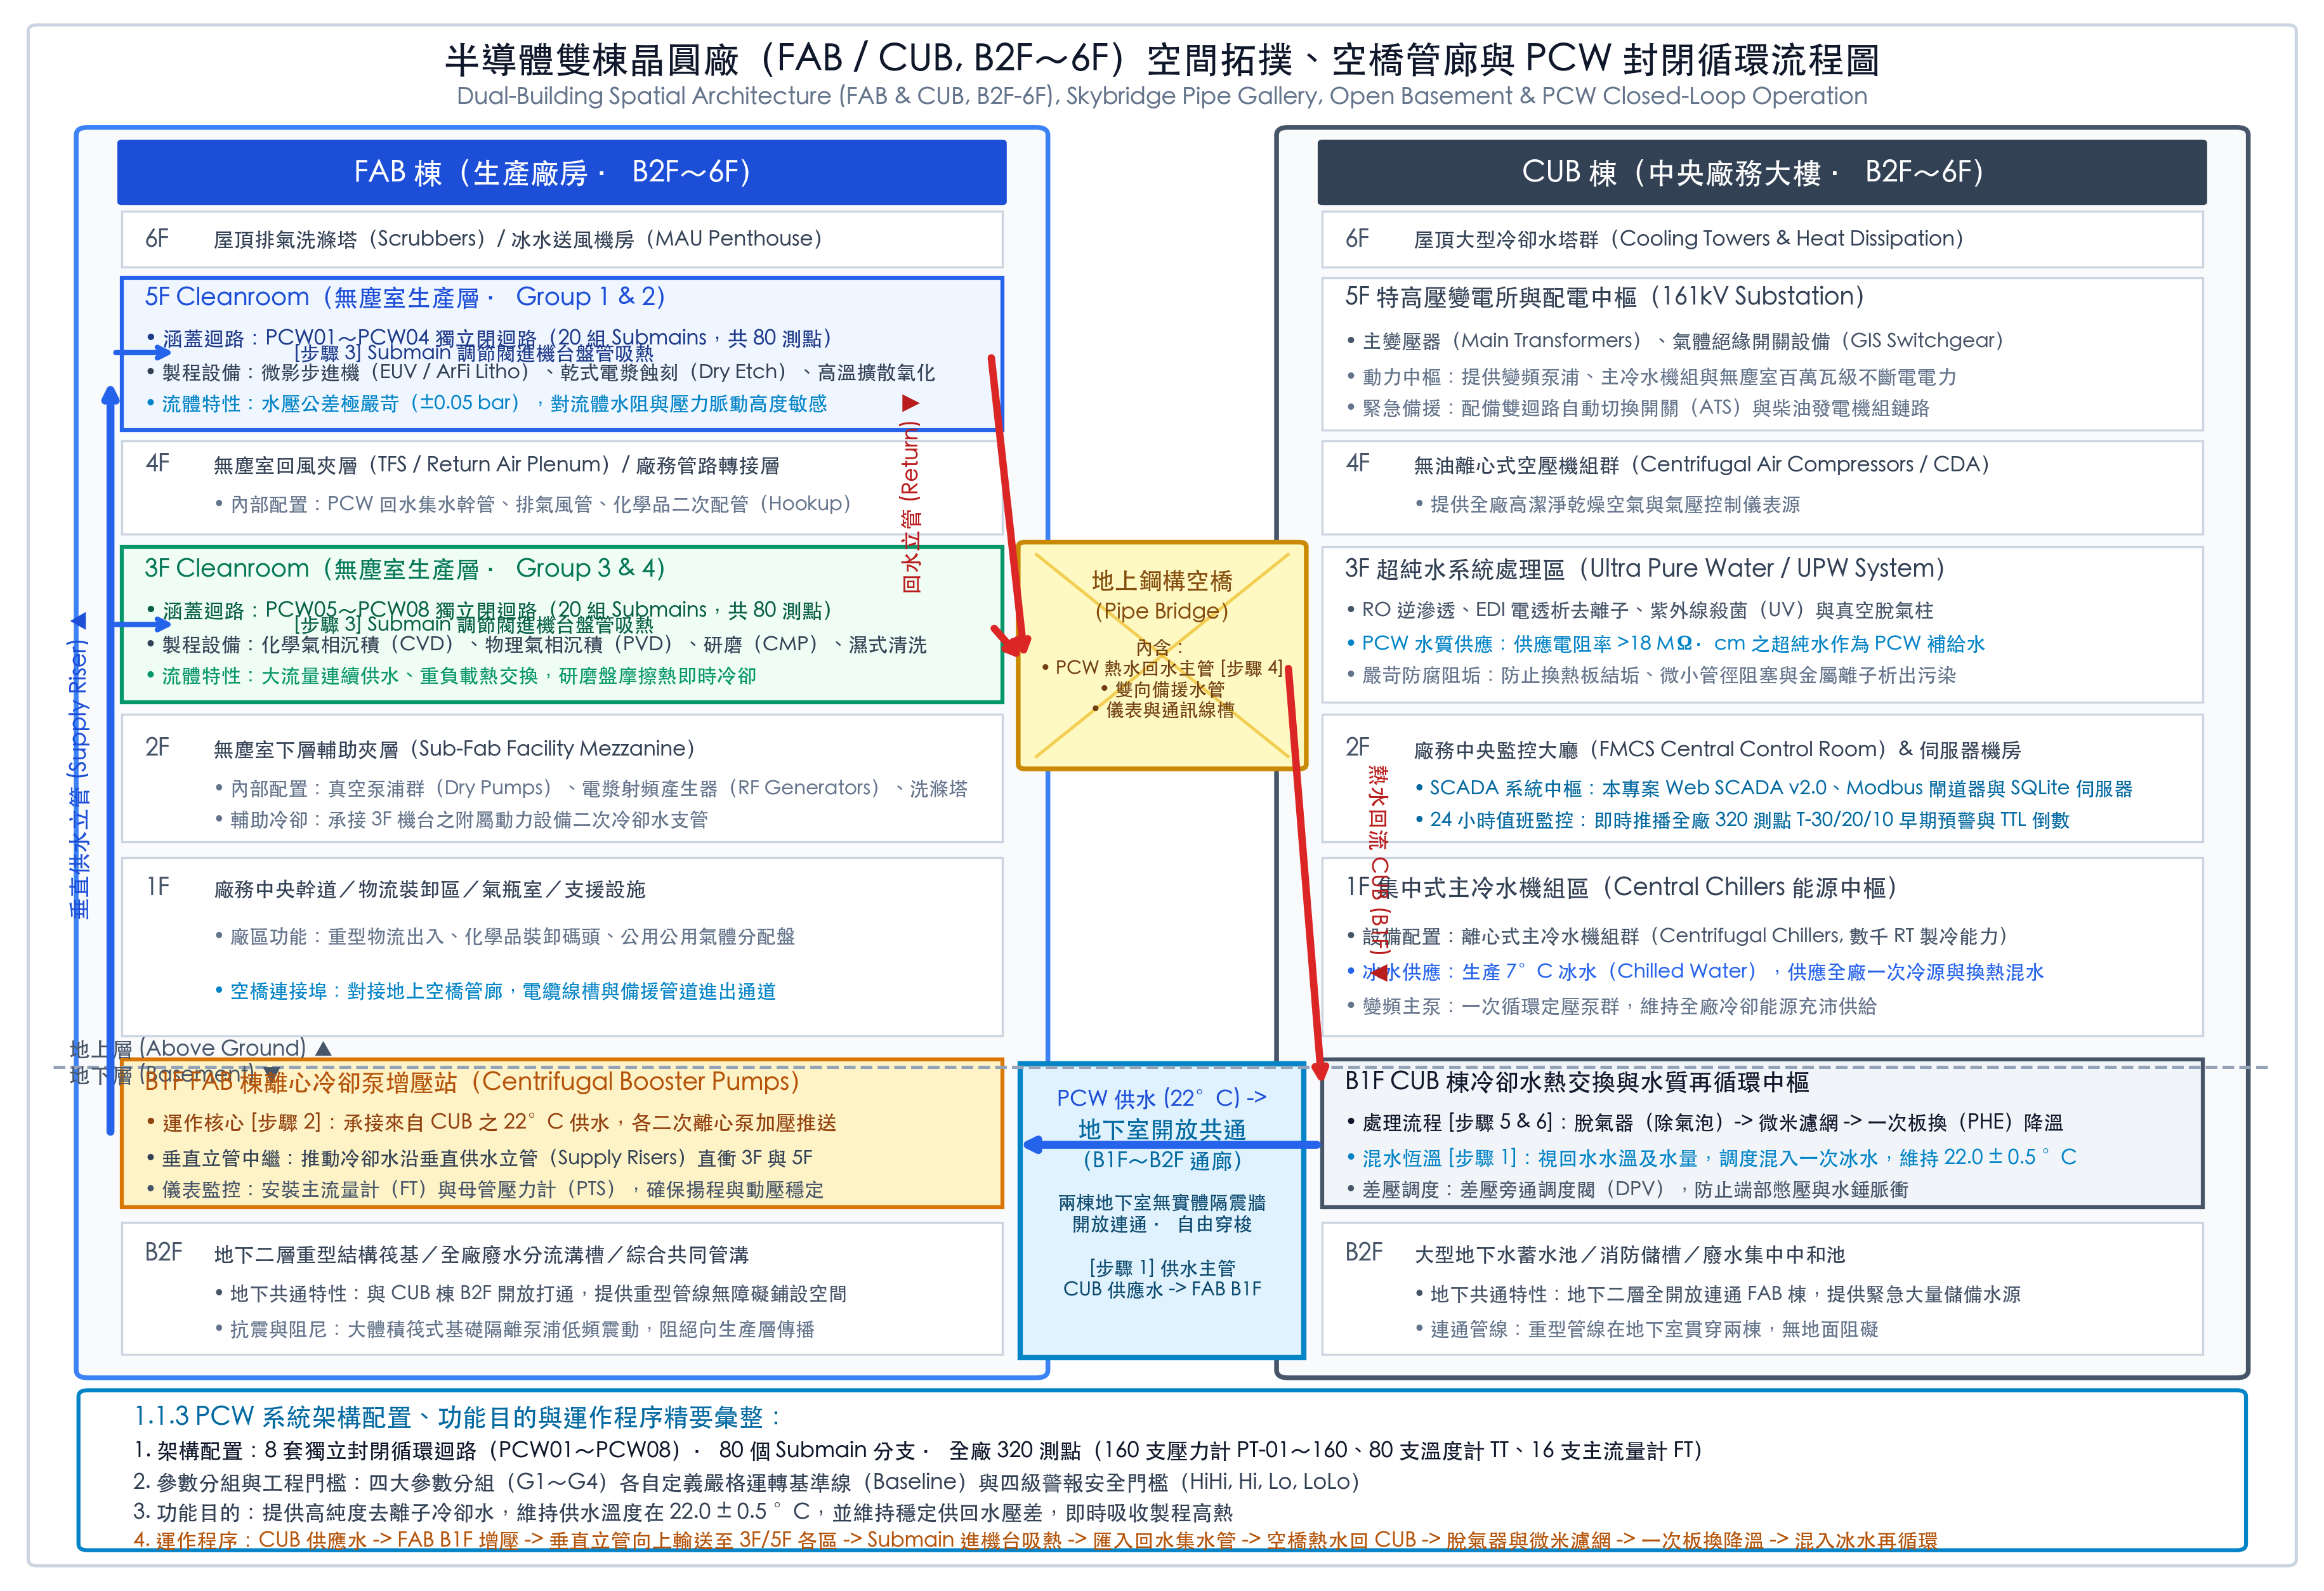
\includegraphics[width=0.92\textwidth,keepaspectratio]{picture/fig_fab_topology_design.png}
    \caption{雙層晶圓廠 PCW01–PCW08 迴路與 320 測點拓撲配置圖}
    \label{fig:fab_topo}
\end{figure}

全廠總計建置 8 套獨立封閉循環迴路（PCW01 至 PCW08），每套迴路轄下 10 組次幹管（Submain01 至 Submain10），合計全廠共 80 組供／回水配對。每組次幹管依工業儀控標準配置 4 支即時感測器：供水壓力計（\texttt{PTS}）、供水流量計（\texttt{FT}）、回水壓力計（\texttt{PTR}）與供回水壓差計（\texttt{PDT}），全廠總計 \textbf{320 支感測器}（包含 \textbf{160 支 PT}、80 支 FT 及 80 支 PDT）。各迴路依負載特性分屬四大參數分組（Group 1–4），其正常運轉基準線與四級工程安全上下限配置如表~\ref{tab:pcw_groups_v2} 所示。

\begin{table}[H]
\centering
\caption{PCW 八套獨立迴路四大參數分組基準線與工程安全限值配置表}
\label{tab:pcw_groups_v2}
\footnotesize
\renewcommand{\arraystretch}{1.15}
\setlength{\tabcolsep}{5pt}
\begin{tabularx}{0.98\textwidth}{ccccccc}
\toprule
\textbf{分組代碼} & \textbf{涵蓋迴路} & \textbf{配置樓層} & \textbf{測點類型} & \textbf{Baseline} & \textbf{LoLo / Lo} & \textbf{Hi / HiHi} \\
\midrule
Group 1 & PCW01, PCW02 & 2F Cleanroom & PT (\texttt{PTS}/\texttt{PTR}) & 1.50 bar & 1.20 / 1.30 & 1.70 / 1.80 \\
Group 2 & PCW03, PCW04 & 2F Cleanroom & PT (\texttt{PTS}/\texttt{PTR}) & 1.90 bar & 1.50 / 1.70 & 2.10 / 2.20 \\
Group 3 & PCW05, PCW06 & 1F Sub-Fab   & PT (\texttt{PTS}/\texttt{PTR}) & 2.50 bar & 2.20 / 2.30 & 2.70 / 2.80 \\
Group 4 & PCW07, PCW08 & 1F Sub-Fab   & PT (\texttt{PTS}/\texttt{PTR}) & 2.20 bar & 1.90 / 2.00 & 2.40 / 2.50 \\
\midrule
Group 1/2 & PCW01–04 & 2F Cleanroom & FT (流量) & 180 LPM & 150 / 160 & 200 / 220 \\
Group 3   & PCW05–06 & 1F Sub-Fab   & FT (流量) & 260 LPM & 230 / 240 & 280 / 300 \\
Group 4   & PCW07–08 & 1F Sub-Fab   & FT (流量) & 240 LPM & 200 / 220 & 260 / 280 \\
All       & PCW01–08 & 1F / 2F      & PDT (壓差) & 0.30 bar & 0.00 / 0.10 & 0.50 / 0.60 \\
\bottomrule
\end{tabularx}
\end{table}

\subsection{研究動機與研究目的}
在現行半導體 SCADA 系統中，警報發布多仰賴靜態工程門檻（HI/HIHI/LO/LOLO）。此機制雖直觀明確，但在實務上面臨兩項痛點：
\begin{enumerate}
    \item \textbf{缺乏事前防禦處置時間}：當靜態警報響起時，物理壓力已突破安全界限，運轉人員僅能被動停機或切換備援泵，常造成晶圓報廢或昂貴機台熱跳脫。
    \item \textbf{緩慢漂移不易識別}：管路因濾網逐漸阻塞、閥門開度偏移或熱負載漸變引發之未越限緩慢漂移，靜態門檻完全無法察覺；而傳統管制圖在生產負載週期波動下易累積虛警。
\end{enumerate}

針對上述問題，本研究以指導教授認可之初版 Excel 驗證模型為設計基礎，確立四大具體研究目的：
\begin{enumerate}
    \item 嚴格定義\textbf{偏移偵測（Drift Detection）}與\textbf{趨勢預測（Trend Forecast）}兩大核心數學模型，在 Past-Only 因果約束下實現無偏早期預警。
    \item 建立全端可重現 Web SCADA 原型系統，整合非同步 Modbus/TCP 工業通訊伺服器、SQLite WAL 歷史庫與即時推播監控介面。
    \item 實施七層工業硬化防線（L1–L7），抑制瞬態突波誤報並保證長時段持續水準偏移下的預警穩定性。
    \item 透過 3,840 場受控基準比較、480 筆歷史回放與 11.35 分鐘全廠實時行為偏差連續實測，完整驗證系統之預警能力、微秒級推論延遲與工程可靠度。
\end{enumerate}

% ============================================================
% 第二章 文獻探討與理論基礎
% ============================================================
\clearpage
\section{文獻探討與理論基礎}

\subsection{工業警報管理標準與預警事件分離}
ANSI/ISA-18.2 工業警報管理標準強調，警報系統必須具備完整的生命週期管理、死區（Deadband）與延遲防抖（On-Delay）設計，以避免操作員遭遇警報疲勞（Alarm Fatigue）~\cite{isa1822016}。本研究據此嚴格實施「預警（$T\text{-}30/20/10$）」與「工程越限事件（\texttt{EVENT}）」之狀態分離：預警旨在爭取黃金處置窗口，而 \texttt{EVENT} 則標記硬體邊界突破。

\subsection{統計製程管制與因果時間序列約束}
統計製程管制（SPC）之指數加權移動平均（EWMA）由 Roberts~\cite{roberts1959control} 提出並由 Montgomery~\cite{montgomery2020statistical} 系統化，具備對微小平均偏移之高靈敏度。但在工業流體監控中，EWMA 僅輸出無因次統計量，無法提供直觀的到限剩餘時間（TTL）。

在機器學習與時序分析中，Kaufman 等人~\cite{kaufman2012leakage} 深入論證資料洩漏（Data Leakage）對離線評估的誤導性。本研究堅持 Past-Only 因果原則：所有推論特徵僅能取自 $[t-W, t)$ 之過去觀測值，絕不引用當前時刻之後之任何數據。流體力學基礎方面，Darcy~\cite{darcy1857recherches} 與 Colebrook~\cite{colebrook1939turbulent} 之管流摩擦阻力理論為供回水壓差分析提供了物理先驗指導。工業通訊協定方面，系統後端依據 Modbus Organization 官方標準規範~\cite{modbus2006spec} 實作完整之 Modbus/TCP MBAP 訊框與保持暫存器服務。

% ============================================================
% 第三章 系統架構與統計式早期預警方法
% ============================================================
\clearpage
\section{系統架構與統計式早期預警方法}

\subsection{五層式軟硬體系統架構}
如圖~\ref{fig:arch_layers} 所示，本系統採五層分層架構設計，涵蓋實體製程層、工業協定層、核心推論引擎層、應用服務層與控制室人機介面層。後端整合純 Python 非同步 Modbus/TCP 伺服器（Port 15020）、SQLite WAL 歷史與推論日誌資料庫、統一推論引擎與 FastAPI 服務，並透過 SSE（Server-Sent Events）即時推播驅動 React 19 全端 Web SCADA。

\begin{figure}[H]
    \centering
    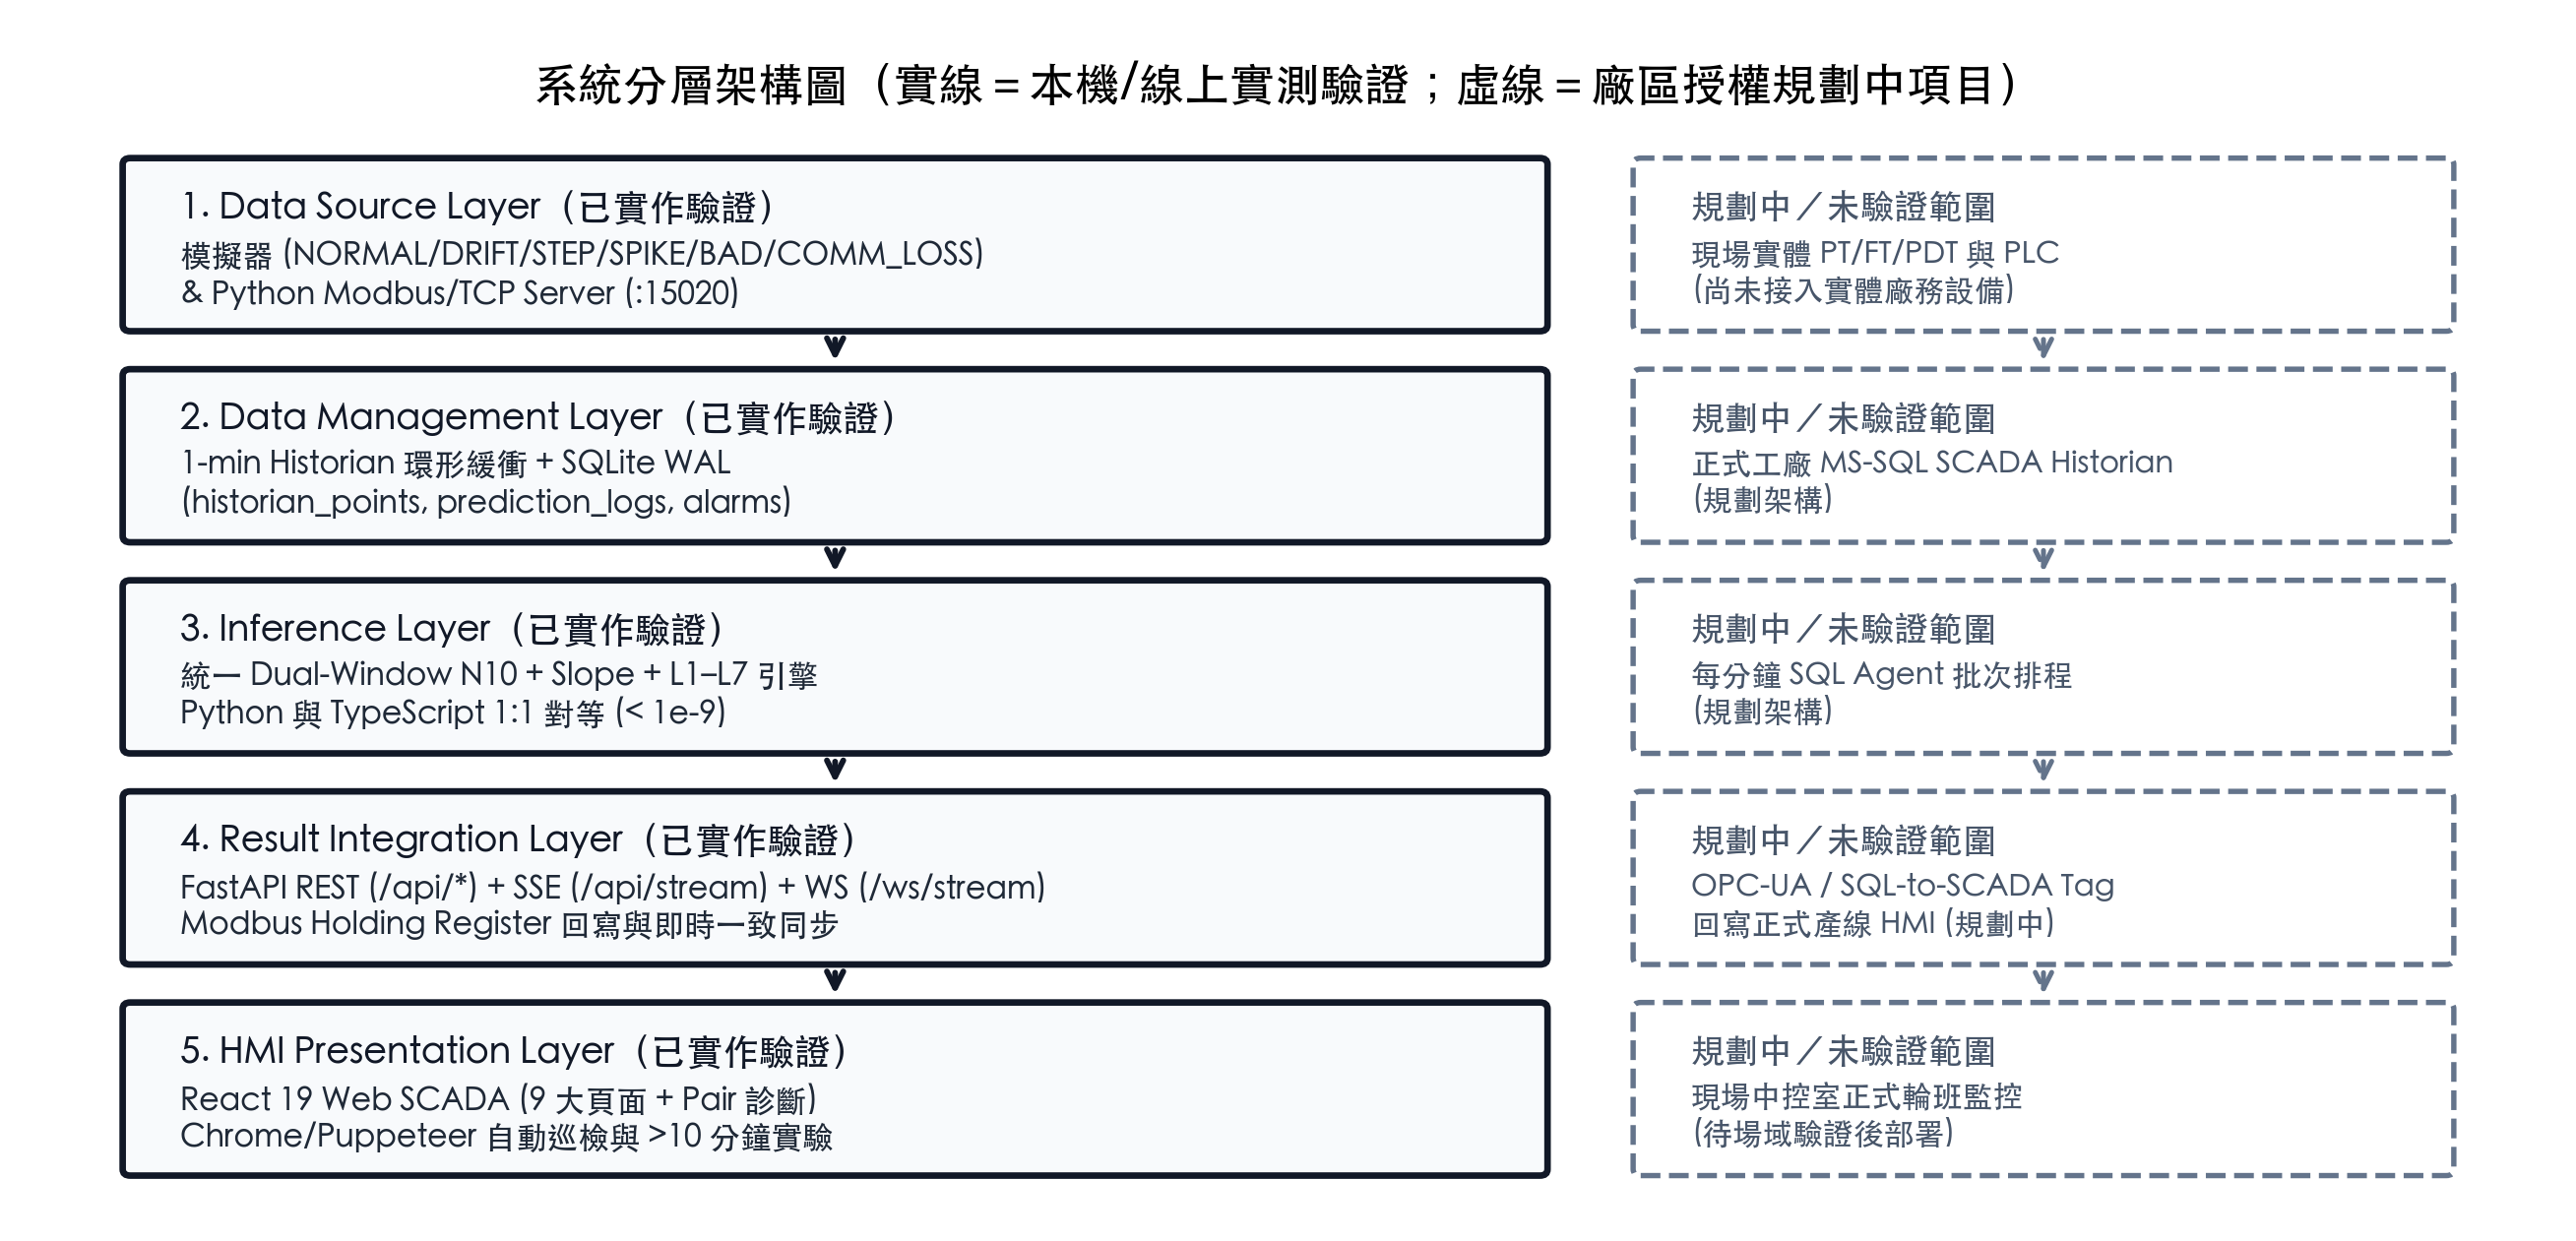
\includegraphics[width=0.95\textwidth,keepaspectratio]{picture/fig_system_architecture_layers.png}
    \caption{五層式軟硬體系統架構圖}
    \label{fig:arch_layers}
\end{figure}

\subsection{Modbus/TCP 保持暫存器映射架構}
全廠 320 支感測器依表~\ref{tab:modbus_map_v2} 連續映射至 Modbus Holding Registers \texttt{40001} 至 \texttt{40639}（共 640 個 16-bit 暫存器）。每支測點採用 IEEE-754 單精度浮點數（FLOAT32）配合 CDAB Word-Swap 位元組順序編碼，完全符合工業 PLC 與 DCS 連線規範。

\begin{table}[H]
\centering
\caption{全廠 320 測點 Modbus/TCP FLOAT32 (CDAB) 保持暫存器位址映射表}
\label{tab:modbus_map_v2}
\footnotesize
\renewcommand{\arraystretch}{1.15}
\setlength{\tabcolsep}{4pt}
\begin{tabularx}{\textwidth}{cccXc}
\toprule
\textbf{迴路代碼} & \textbf{暫存器位址範圍} & \textbf{次幹管涵蓋} & \textbf{測點類型與數量} & \textbf{資料編碼格式} \\
\midrule
PCW01 & 40001 -- 40079 & Submain01--10 & 20 PT, 10 FT, 10 PDT (40 點) & FLOAT32 CDAB \\
PCW02 & 40081 -- 40159 & Submain01--10 & 20 PT, 10 FT, 10 PDT (40 點) & FLOAT32 CDAB \\
PCW03 & 40161 -- 40239 & Submain01--10 & 20 PT, 10 FT, 10 PDT (40 點) & FLOAT32 CDAB \\
PCW04 & 40241 -- 40319 & Submain01--10 & 20 PT, 10 FT, 10 PDT (40 點) & FLOAT32 CDAB \\
PCW05 & 40321 -- 40399 & Submain01--10 & 20 PT, 10 FT, 10 PDT (40 點) & FLOAT32 CDAB \\
PCW06 & 40401 -- 40479 & Submain01--10 & 20 PT, 10 FT, 10 PDT (40 點) & FLOAT32 CDAB \\
PCW07 & 40481 -- 40559 & Submain01--10 & 20 PT, 10 FT, 10 PDT (40 點) & FLOAT32 CDAB \\
PCW08 & 40561 -- 40639 & Submain01--10 & 20 PT, 10 FT, 10 PDT (40 點) & FLOAT32 CDAB \\
\bottomrule
\end{tabularx}
\end{table}

\subsection{Excel 初版模型設計基礎與 Past-Only 因果滑動視窗}
本系統演算法以獲指導教授認可之初版 Excel 驗證模型（\texttt{PCW\_T30\_T20\_T10\_FINAL\_ROLLBACK}）為設計基礎，確立了\textbf{偏移偵測（Drift Detection）}與\textbf{趨勢預測（Trend Forecast）}雙核心架構。

如圖~\ref{fig:window_design} 所示，於任意推論時刻 $t$，系統僅讀取過去 70 分鐘已結算之觀測值，劃分為三個因果互斥區間：
\begin{enumerate}
    \item \textbf{歷史基準區間（60 分鐘）}：$[t-70, t-10)$，建立該測點近期之正常穩態參考值（$\mathrm{BaseAvg}_{60}$）。
    \item \textbf{前期局部區間（5 分鐘）}：$[t-10, t-5)$，作為計算近期變化斜率的起始平均基準（$\mathrm{Prev5Avg}$）。
    \item \textbf{近期局部區間（5 分鐘）}：$[t-5, t)$，作為計算近期變化斜率的終點平均基準（$\mathrm{Recent5Avg}$）；前後兩段 5 分鐘合併即為近期 10 分鐘觀察區間 $[t-10, t)$。
\end{enumerate}

\begin{figure}[H]
    \centering
    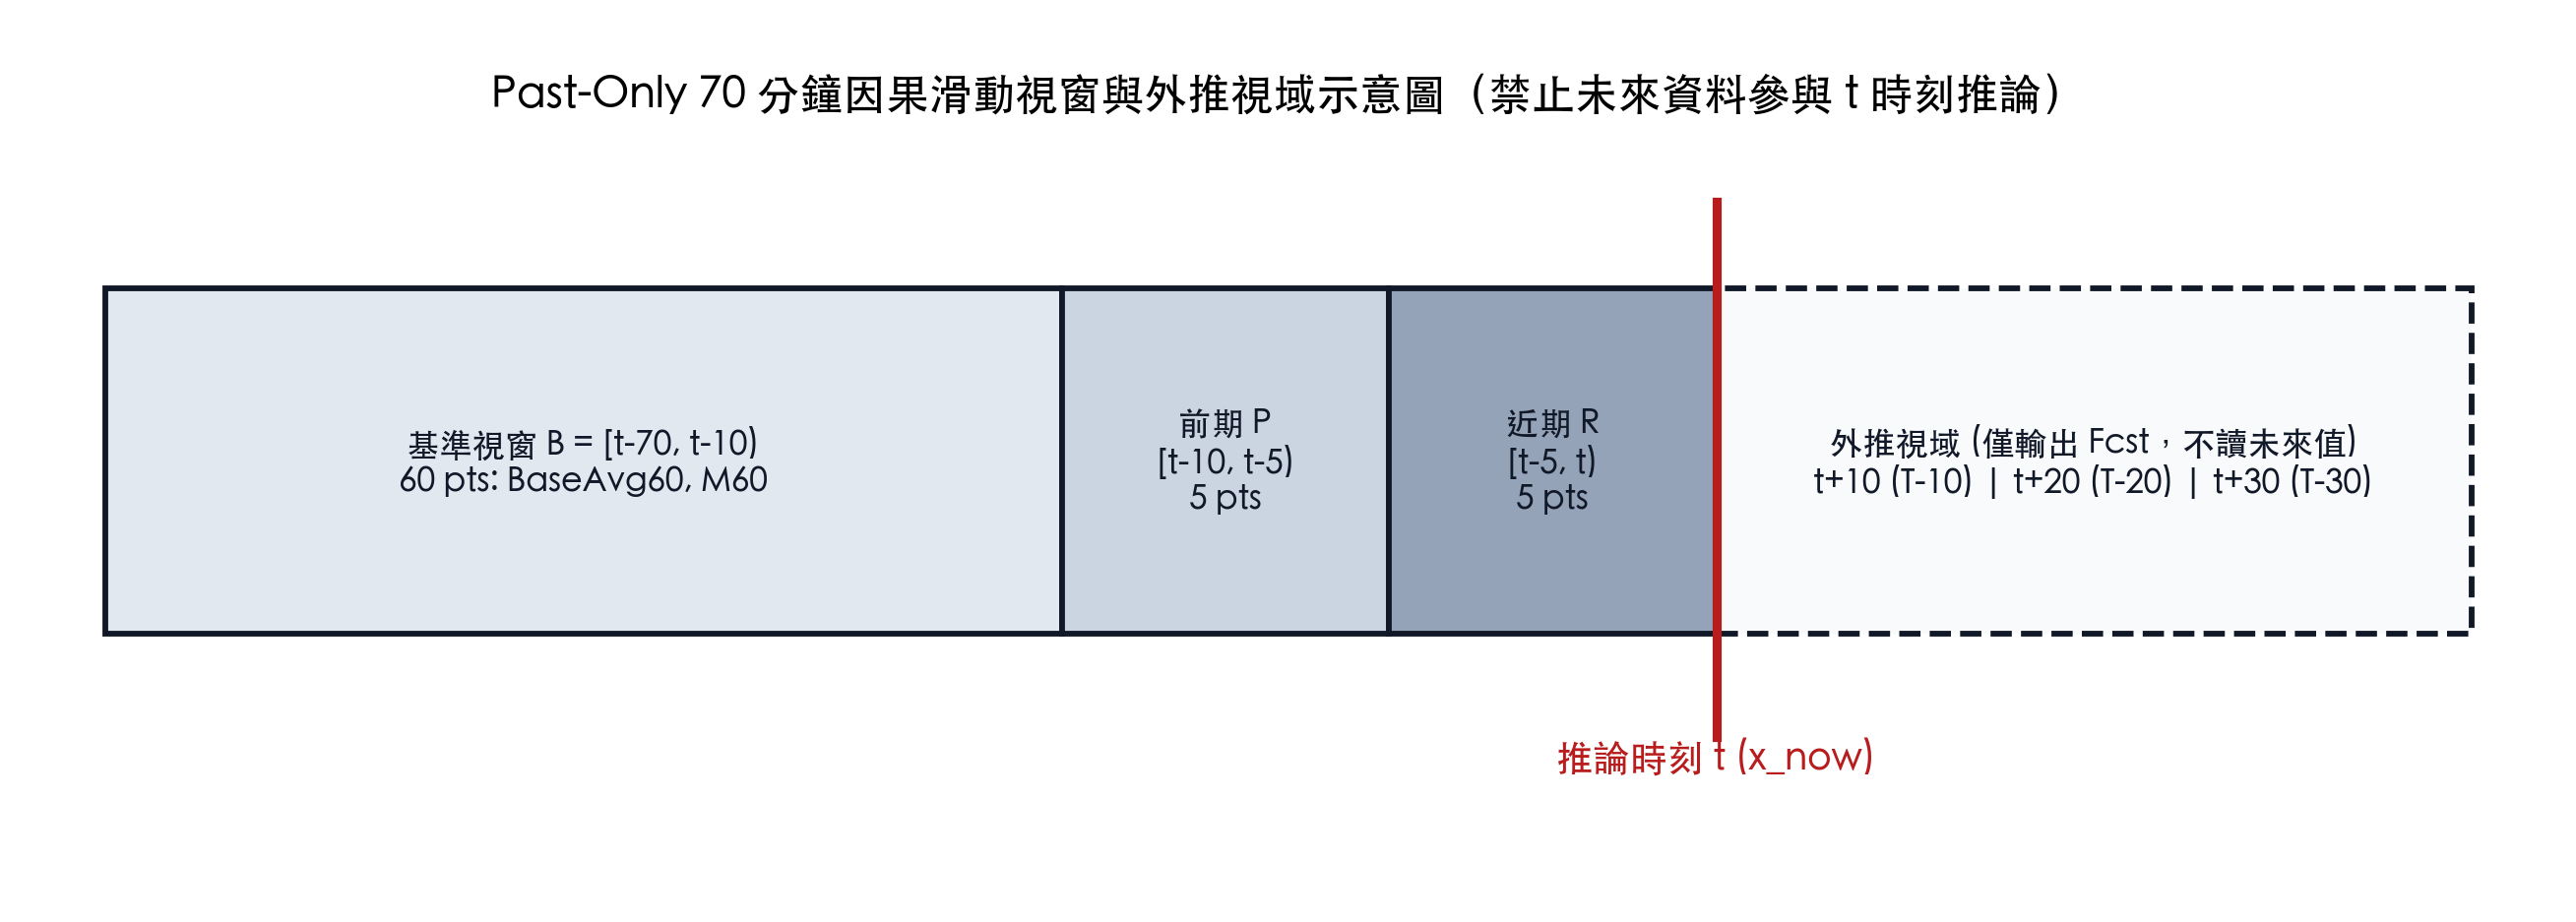
\includegraphics[width=0.92\textwidth,keepaspectratio]{picture/fig_past_only_window_design.png}
    \caption{Past-Only 70 分鐘因果滑動視窗切分與多視域外推示意圖}
    \label{fig:window_design}
\end{figure}

表~\ref{tab:excel_to_program_map} 彙整初版 Excel 模型與本系統 Unified V1 演算法之對應關係。

\begin{table}[H]
\centering
\caption{初版 Excel 參考模型與系統 Unified V1 核心演算法對照表}
\label{tab:excel_to_program_map}
\scriptsize
\renewcommand{\arraystretch}{1.2}
\setlength{\tabcolsep}{3.5pt}
\begin{tabularx}{\textwidth}{>{\bfseries}l l X X}
\toprule
核心問題 & Excel 欄位 / 參數 & Excel 初版設計（單向上漂） & 系統 Unified V1 實作（雙向 / 全廠 320 點） \\
\midrule
事件界限 & \texttt{D4} (\texttt{AlarmLimit}) & 讀值 $\ge 1.70$ 即判定為 \texttt{EVENT} & 讀值 $\ge H_i$ 或 $\le L_i$ 即判定為 \texttt{EVENT}（L5 事件分離） \\
偏移偵測 & \texttt{K4} (\texttt{BaseAvg60}) & 過去 60 分鐘 $[t-70,t-10)$ 平均值 & 嚴格計入 \texttt{GOOD} 樣本，基準期需滿 30 點（L1 品質檢核） \\
偏移偵測 & \texttt{L4, M4} (\texttt{M60, M10}) & 區間內大於基準值之偏高筆數 & 依斜率方向動態統計同向偏離筆數，支援滿窗還原（式~\eqref{eq:m60_m10}） \\
偏移偵測 & \texttt{N4} (\texttt{N10}) & 密度倍比 $N_{10} = M_{10}/(M_{60}/6)$ & 無因次倍率計算式~\eqref{eq:n10}，判定門檻採 $N_{10} \ge \theta$ \\
偏移偵測 & \texttt{Gate30/20/10} & 固定水位門檻 $\{1.55, 1.58, 1.62\}$ & 通用跨度水準偏移閘門 $\ge g\%\times(H_i-L_i)$（式~\eqref{eq:drift_gate}） \\
趨勢預測 & \texttt{E4, F4} (\texttt{P5, R5}) & $[t-10,t-5)$ 與 $[t-5,t)$ 均值 & 兩段 5 分鐘有效樣本均值 $\mathrm{Prev5Avg}$ 與 $\mathrm{Recent5Avg}$ \\
趨勢預測 & \texttt{G4} (\texttt{Slope/min}) & $\max\bigl(0, (\mathrm{R5}-\mathrm{P5})/5\bigr)$ & 保留雙向斜率 $(\mathrm{Recent5}-\mathrm{Prev5})/5$（式~\eqref{eq:base_slope}） \\
趨勢預測 & \texttt{H4:J4} (\texttt{Forecast}) & 目前值 $+$ 斜率 $\times\ h$ 分鐘 & 雙向線性外推 $+$ OLS 95\% 信賴錐面 $+$ 到限時間 $\mathrm{TTL}$ \\
聯合決策 & \texttt{O4:Q4} (\texttt{Pred\_T*}) & （外推越限）或（$N_{10}$ 成立且達標） & （外推越限）或（偏移成立）$+$ 前置防抖確認（L6） \\
\bottomrule
\end{tabularx}
\end{table}

\noindent\textbf{【口試備註：為何固定切 60 分鐘基準與 10 分鐘近期，不看即時那 1 分鐘？】}\\
口試簡答：「因為嚴格遵守因果約束，絕不偷看未來資料；60 分鐘長度足以代表正常工況穩態基準，而前後兩段 5 分鐘均值能有效濾除單點高頻雜訊波動。」

\subsection{核心模型一：偏移偵測數學公式 (Drift Detection Model)}
\label{sec:drift_detection}
偏移偵測模型旨在解決：壓力數值尚未觸碰固定警報線（如 $1.70\ \mathrm{bar}$），但已顯著偏離過去一小時常態水位且持續不退之微幅行為偏移。

\subsubsection{雙視窗異常密度比基礎公式}
演算法依據變化方向統計基準期與近期區間之偏離筆數：
\begin{align}
\mathrm{BaseAvg}_{60}(t) &= \frac{1}{|I_{60}|} \sum_{k \in I_{60}} x(k), \qquad I_{60} = [t-70, t-10) \nonumber \\
M_{60}(t) &= \mathrm{round}\!\left(\text{基準區間同向偏離個數} \times \frac{60}{\text{基準有效點數}}\right) \nonumber \\
M_{10}(t) &= \mathrm{round}\!\left(\text{近 10 分區間同向偏離個數} \times \frac{10}{\text{近期有效點數}}\right)
\label{eq:m60_m10}
\end{align}
由於 60 分鐘為 10 分鐘的 6 倍，常態下 10 分鐘內的預期偏離筆數為 $M_{60}/6$。定義無因次異常密度比 $N_{10}$ 如下：
\begin{equation}
N_{10}(t) = \begin{cases}
\dfrac{M_{10}(t)}{M_{60}(t) \div 6}, & \text{當 } M_{60}(t) > 0 \\[8pt]
999, & \text{當 } M_{60}(t)=0 \text{ 且 } M_{10}(t)>0 \\
0, & \text{當 } M_{60}(t)=0 \text{ 且 } M_{10}(t)=0
\end{cases}
\label{eq:n10}
\end{equation}

\subsubsection{通用跨度水準偏移閘門與防禦條件}
為使模型通用於全廠不同量程之感測器（PT、FT、PDT），並確保在長時段穩態偏移下（局部斜率趨近 0）仍能持續鎖定預警，定義操作跨度 $S_i = H_i - L_i$，以及近期均值相對於基準均值之水準位移差 $\Delta\mu_{10}(t) = |\mathrm{Avg}_{10}(t) - \mathrm{BaseAvg}_{60}(t)|$。偏移偵測成立之充分必要條件定義為：
\begin{equation}
\text{偏移偵測成立} \iff \bigl(N_{10}(t) \ge \theta\bigr) \;\text{且}\; \Bigl(|\mathrm{Slope}(t)\times 30| \ge \frac{g}{100}S_i \;\text{或}\; \Delta\mu_{10}(t) \ge \frac{g}{100}S_i\Bigr)
\label{eq:drift_gate}
\end{equation}
系統基準設定值為靈敏度 $\theta = 2.0$、跨度比例門檻 $g = 5.0\%$。

\noindent\textbf{【口試備註：演算法設定 $N_{10} \ge 2$ 與增加水準位移項的物理意義？】}
\begin{enumerate}
    \item \textbf{為什麼門檻採用 $N_{10} \ge 2$？} 在常態雜訊對稱分佈下（$M_{60} \ge 30$），即使近 10 分鐘全數異常（$M_{10}=10$），比值上限恰為 $10 \div (30/6) = 2.0$。若使用嚴格大於門檻將導致極限情況無法觸發，故採用 $\ge \theta$ 保證數學完整覆蓋。
    \item \textbf{為什麼加入水準位移項 $\Delta\mu_{10}$？} 當異常偏移維持超過 10 分鐘後，前後兩段 5 分鐘均值皆處於高檔，相減得出之局部斜率會收斂歸零。引入長時段水準位移差 $\Delta\mu_{10}$，能保證在持續穩態偏差工況下穩定發布預警，避免誤解除。
\end{enumerate}

\subsection{核心模型二：趨勢預測數學公式 (Trend Forecast Model)}
\label{sec:trend_forecast}
趨勢預測模型旨在評估：若依當前水壓變化速率外推，未來 10、20、30 分鐘是否會越界？剩餘處置時間（TTL）為何？預測值之信賴區間有多寬？

\subsubsection{前後均差斜率與多時域外推}
為避免單分鐘雜訊對數值微分造成擾動放大，演算法先計算前後兩段 5 分鐘之平滑均值，再計算單位時間斜率並進行外推：
\begin{align}
\mathrm{Prev5Avg}(t) &= \frac{1}{5} \sum_{k=1}^5 x(t-10+k), \qquad
\mathrm{Recent5Avg}(t) = \frac{1}{5} \sum_{k=1}^5 x(t-5+k) \nonumber \\
\mathrm{Slope}(t) &= \frac{\mathrm{Recent5Avg}(t) - \mathrm{Prev5Avg}(t)}{5} \nonumber \\
\hat{x}(t+h) &= x_{\mathrm{now}} + \mathrm{Slope}(t) \times h \qquad (h\in\{10,20,30\})
\label{eq:base_slope}
\end{align}
只要外推值 $\hat{x}(t+h) \ge H_i$ 或 $\le L_i$，即觸發對應視域之預警。

\subsubsection{OLS 95\% 預測信賴區間與閉式到限時間 (TTL)}
為向操作人員呈現預測不確定性，系統對近 $n=10$ 分鐘序列擬合普通最小平方法（OLS）回歸線 $\hat{y}(h) = a + b \cdot h$，計算殘差標準差 $s_e$：
\begin{equation}
s_e = \sqrt{\frac{\sum_{i=1}^n (y_i - \hat{y}_i)^2}{n - 2}}
\end{equation}
依 Student-$t$ 分佈（$n=10$ 自由度為 8 時，$t_{0.975,8} = 2.306$），得出未來第 $h$ 分鐘之 95\% 預測半寬 $\delta_h$：
\begin{equation}
\delta_h = 2.306 \times s_e \times \sqrt{1 + \frac{1}{n} + \frac{(h - \bar{h})^2}{\sum (h_k - \bar{h})^2}}
\label{eq:pred_band}
\end{equation}
在介面上呈現隨外推時間逐漸擴展之風險錐面（$\hat{y}(h) \pm \delta_h$）。

同時，令 $U^*$ 為目標方向之工程門檻，計算剩餘到限時間（TTL）：
\begin{equation}
\mathrm{TTL}(t) = \frac{U^* - x_{\mathrm{now}}}{\mathrm{Slope}(t)}
\label{eq:ttl}
\end{equation}

\noindent\textbf{【口試備註：OLS 預測錐面與均差斜率外推的分工？】}\\
口試簡答：「五分鐘均差斜率 $\mathrm{Slope}$ 負責穩定輸出中心預測軌跡；而近 10 點 OLS 回歸則計算 95\% Student-$t$ 預測半寬 $\delta_h$，在 Web SCADA 畫面上形成隨外推時間漸寬的信心錐面，讓操作員一目了然預測的可信度範圍。」

\subsection{七層工業級硬化決策與演算法流程}
本系統整合七層工業硬化防線（L1–L7），確保在複雜工況下的決策嚴謹性：
\begin{itemize}
    \item \textbf{L1 數據品質閘門}：僅計入 \texttt{GOOD} 樣本，有效率低於 $80\%$ 即回傳 \texttt{INSUFFICIENT\_DATA}。
    \item \textbf{L2 雙重偏移偵測}：結合異常密度倍比 $N_{10}$ 與水準位移差 $\Delta\mu_{10}$。
    \item \textbf{L3 不確定性量化}：OLS 95\% 預測信賴區間動態評估。
    \item \textbf{L4 剩餘時間估算}：閉式 TTL 倒數計算。
    \item \textbf{L5 警報事件分離}：當前值已越界時強制歸入 \texttt{EVENT}，不混入早期預警。
    \item \textbf{L6 前置確認與遲滯鎖存}：支援 $\text{raw\_onset} \in \{1, 2\}$ 連續觸發確認，解除預警需連續 $K_{\mathrm{hold}}=3$ 次安全。
    \item \textbf{L7 多維風險評分}：綜合距限距離、TTL 緊迫度與異常密度輸出 $R_i \in [0, 100]$ 分數。
\end{itemize}

核心推論流程如演算法~\ref{alg:unified_v1} 所示。

\begin{algorithm}[H]
\caption{統一偏移偵測與趨勢預測七層工業硬化演算法 (Unified V1)}
\label{alg:unified_v1}
\begin{algorithmic}[1]
\Require 過去 70 分鐘歷史資料、目前讀值 $x_{\mathrm{now}}$、安全上下限 $(L, H)$、參數 $(\theta, g, K_{\mathrm{hold}}, \text{raw\_onset})$
\Ensure 偏移指標（$\mathrm{BaseAvg}_{60}, M_{60}, M_{10}, N_{10}, \Delta\mu_{10}$）與預警決策（$\mathrm{Slope}, \hat{x}_{t+h}, \delta_h, \mathrm{TTL}, S_i, R_i$）
\State 執行 L1 品質檢核，有效率 $<80\%$ 或基準 $<30$ 點時回傳 \texttt{INSUFFICIENT\_DATA}
\State 計算基準均值 $\mathrm{BaseAvg}_{60}$ 與前後 5 分鐘均值，得出雙向局部斜率 $\mathrm{Slope}$ \Comment{式~\eqref{eq:base_slope}}
\State 依變化方向統計 $M_{60}, M_{10}$，計算異常密度倍比 $N_{10}$ \Comment{式~\eqref{eq:m60_m10}--\eqref{eq:n10}}
\State 評估式~\eqref{eq:drift_gate}，判定偏移偵測是否成立 \Comment{L2 水準偏移保護}
\State 計算多視域外推值 $\hat{x}_{t+h}$、OLS 95\% 信賴半寬 $\delta_h$ 與剩餘時間 $\mathrm{TTL}$ \Comment{L3, L4}
\If{$x_{\mathrm{now}} \ge H$ \textbf{or} $x_{\mathrm{now}} \le L$} $S_{\mathrm{raw}} \leftarrow \texttt{EVENT}$ \Comment{L5 硬事件分離}
\ElsIf{$\hat{x}_{t+10}$ 觸限} $S_{\mathrm{raw}} \leftarrow \texttt{T-10}$
\ElsIf{$\hat{x}_{t+20}$ 觸限} $S_{\mathrm{raw}} \leftarrow \texttt{T-20}$
\ElsIf{$\hat{x}_{t+30}$ 觸限 \textbf{or} 偏移偵測成立} $S_{\mathrm{raw}} \leftarrow \texttt{T-30}$
\Else\ $S_{\mathrm{raw}} \leftarrow \texttt{NORMAL}$
\EndIf
\State 套用 L6 前置確認 ($\text{raw\_onset}$) 與 3 次降級鎖存，輸出狀態 $S_i$ 與風險分數 $R_i$
\end{algorithmic}
\end{algorithm}

\noindent\textbf{【口試備註：如何向口試委員證明演算法無資料洩漏（Zero Data Leakage）？】}\\
口試簡答：「推論演算法所使用的特徵輸入，嚴格限制在推論時刻 $t$ 以前已結算的 70 分鐘資料內；離線驗證所使用的地面真相（未來 $h$ 分鐘是否真實越界）與提前量計算僅在實驗分析腳本中執行，即時線上系統完全無涉未來資料。」

% ============================================================
% 第四章 實驗設計、系統實測與結果分析
% ============================================================
\clearpage
\section{實驗設計、系統實測與結果分析}

\subsection{實測硬體環境與資料集性質}
所有基準評測、微秒級延遲測試與瀏覽器自動化驗證均在統一硬體平台上實施，表~\ref{tab:env_real} 彙整實機探測之軟硬體規格。必須說明的是：除 Excel \texttt{PT-1} 480 分鐘歷史回放為既有基準資料外，全廠 320 測點橫向評測及 11.35 分鐘連續實測均為受控故障注入與模擬器序列，旨在驗證演算法與系統之行為正確性與即時性能。

\begin{table}[H]
\centering
\caption{實測硬體平台、軟體執行環境與資料集規格清冊}
\label{tab:env_real}
\footnotesize
\renewcommand{\arraystretch}{1.15}
\setlength{\tabcolsep}{5pt}
\begin{tabularx}{0.96\textwidth}{>{\bfseries}lX}
\toprule
項目維度 & 實機探測規格與執行版本 \\
\midrule
處理器與記憶體 & Apple M5（10 核心 CPU），16 GiB RAM（17,179,869,184 bytes），ARM64 \\
作業系統與核心 & macOS 26.7.3 (Build 25G342), Darwin Kernel 25.6.0 \\
後端推論環境 & Python 3.9.6, FastAPI 0.115.0, Uvicorn 0.30.6, SQLite 3 (WAL), NumPy 2.0.2 \\
前端與自動化 & Node.js v24.14.1, React 19.2.8, Vite 8.3.0, Google Chrome 157.0.8103.40, Puppeteer 25.13.0 \\
工業通訊協定 & 非同步 Modbus/TCP Server（Port 15020, Unit ID 1, FC03/06/16, FLOAT32 CDAB） \\
系統服務網址 & Web SCADA 控制室介面：\url{http://127.0.0.1:8000/} \\
歷史回放資料集 & Excel \texttt{RawData} 工作表（\texttt{PT-1}，480 分鐘連續觀測序列） \\
全廠測試矩陣 & 320 測點（含 160 PT）$\times$ 12 情境 = 3,840 場固定隨機種子試驗 \\
\bottomrule
\end{tabularx}
\end{table}

\subsection{Excel 初版模型一致性與跨語言數值對等驗證}
為確保程式實作與初版模型完全對齊，本研究首先對 Excel 參考工作簿之 480 筆歷史數據進行逐筆回放重算對比，並檢核 Python 後端與 TypeScript 前端運算之跨語言一致性：
\begin{enumerate}
    \item \textbf{Excel 逐筆比對一致性}：全數 480 筆推論結果比對完全一致（一致率 \textbf{100.00\%}，最大絕對誤差 \textbf{0.0}），如圖~\ref{fig:excel_replay} 所示。在該 480 筆樣本中，首起越限事件發生於 $t=05:08$，系統提前 9.0 分鐘發布 \texttt{T-10} 預警；排除暖機期後之未越限序列實測指標為 Precision=10.17\%、Recall=40.00\%，完整反映單測點歷史數據中存在多次未越限短暫波動之真實特性。
    \item \textbf{跨語言數值對等性}：Python 後端與 TypeScript 前端在常態、慢速漂移、突發越限與品質異常等多種情境下，所有浮點特徵運算誤差皆小於 $10^{-9}$（自動化單元測試 6/6 全數通過）。
\end{enumerate}

\begin{figure}[H]
    \centering
    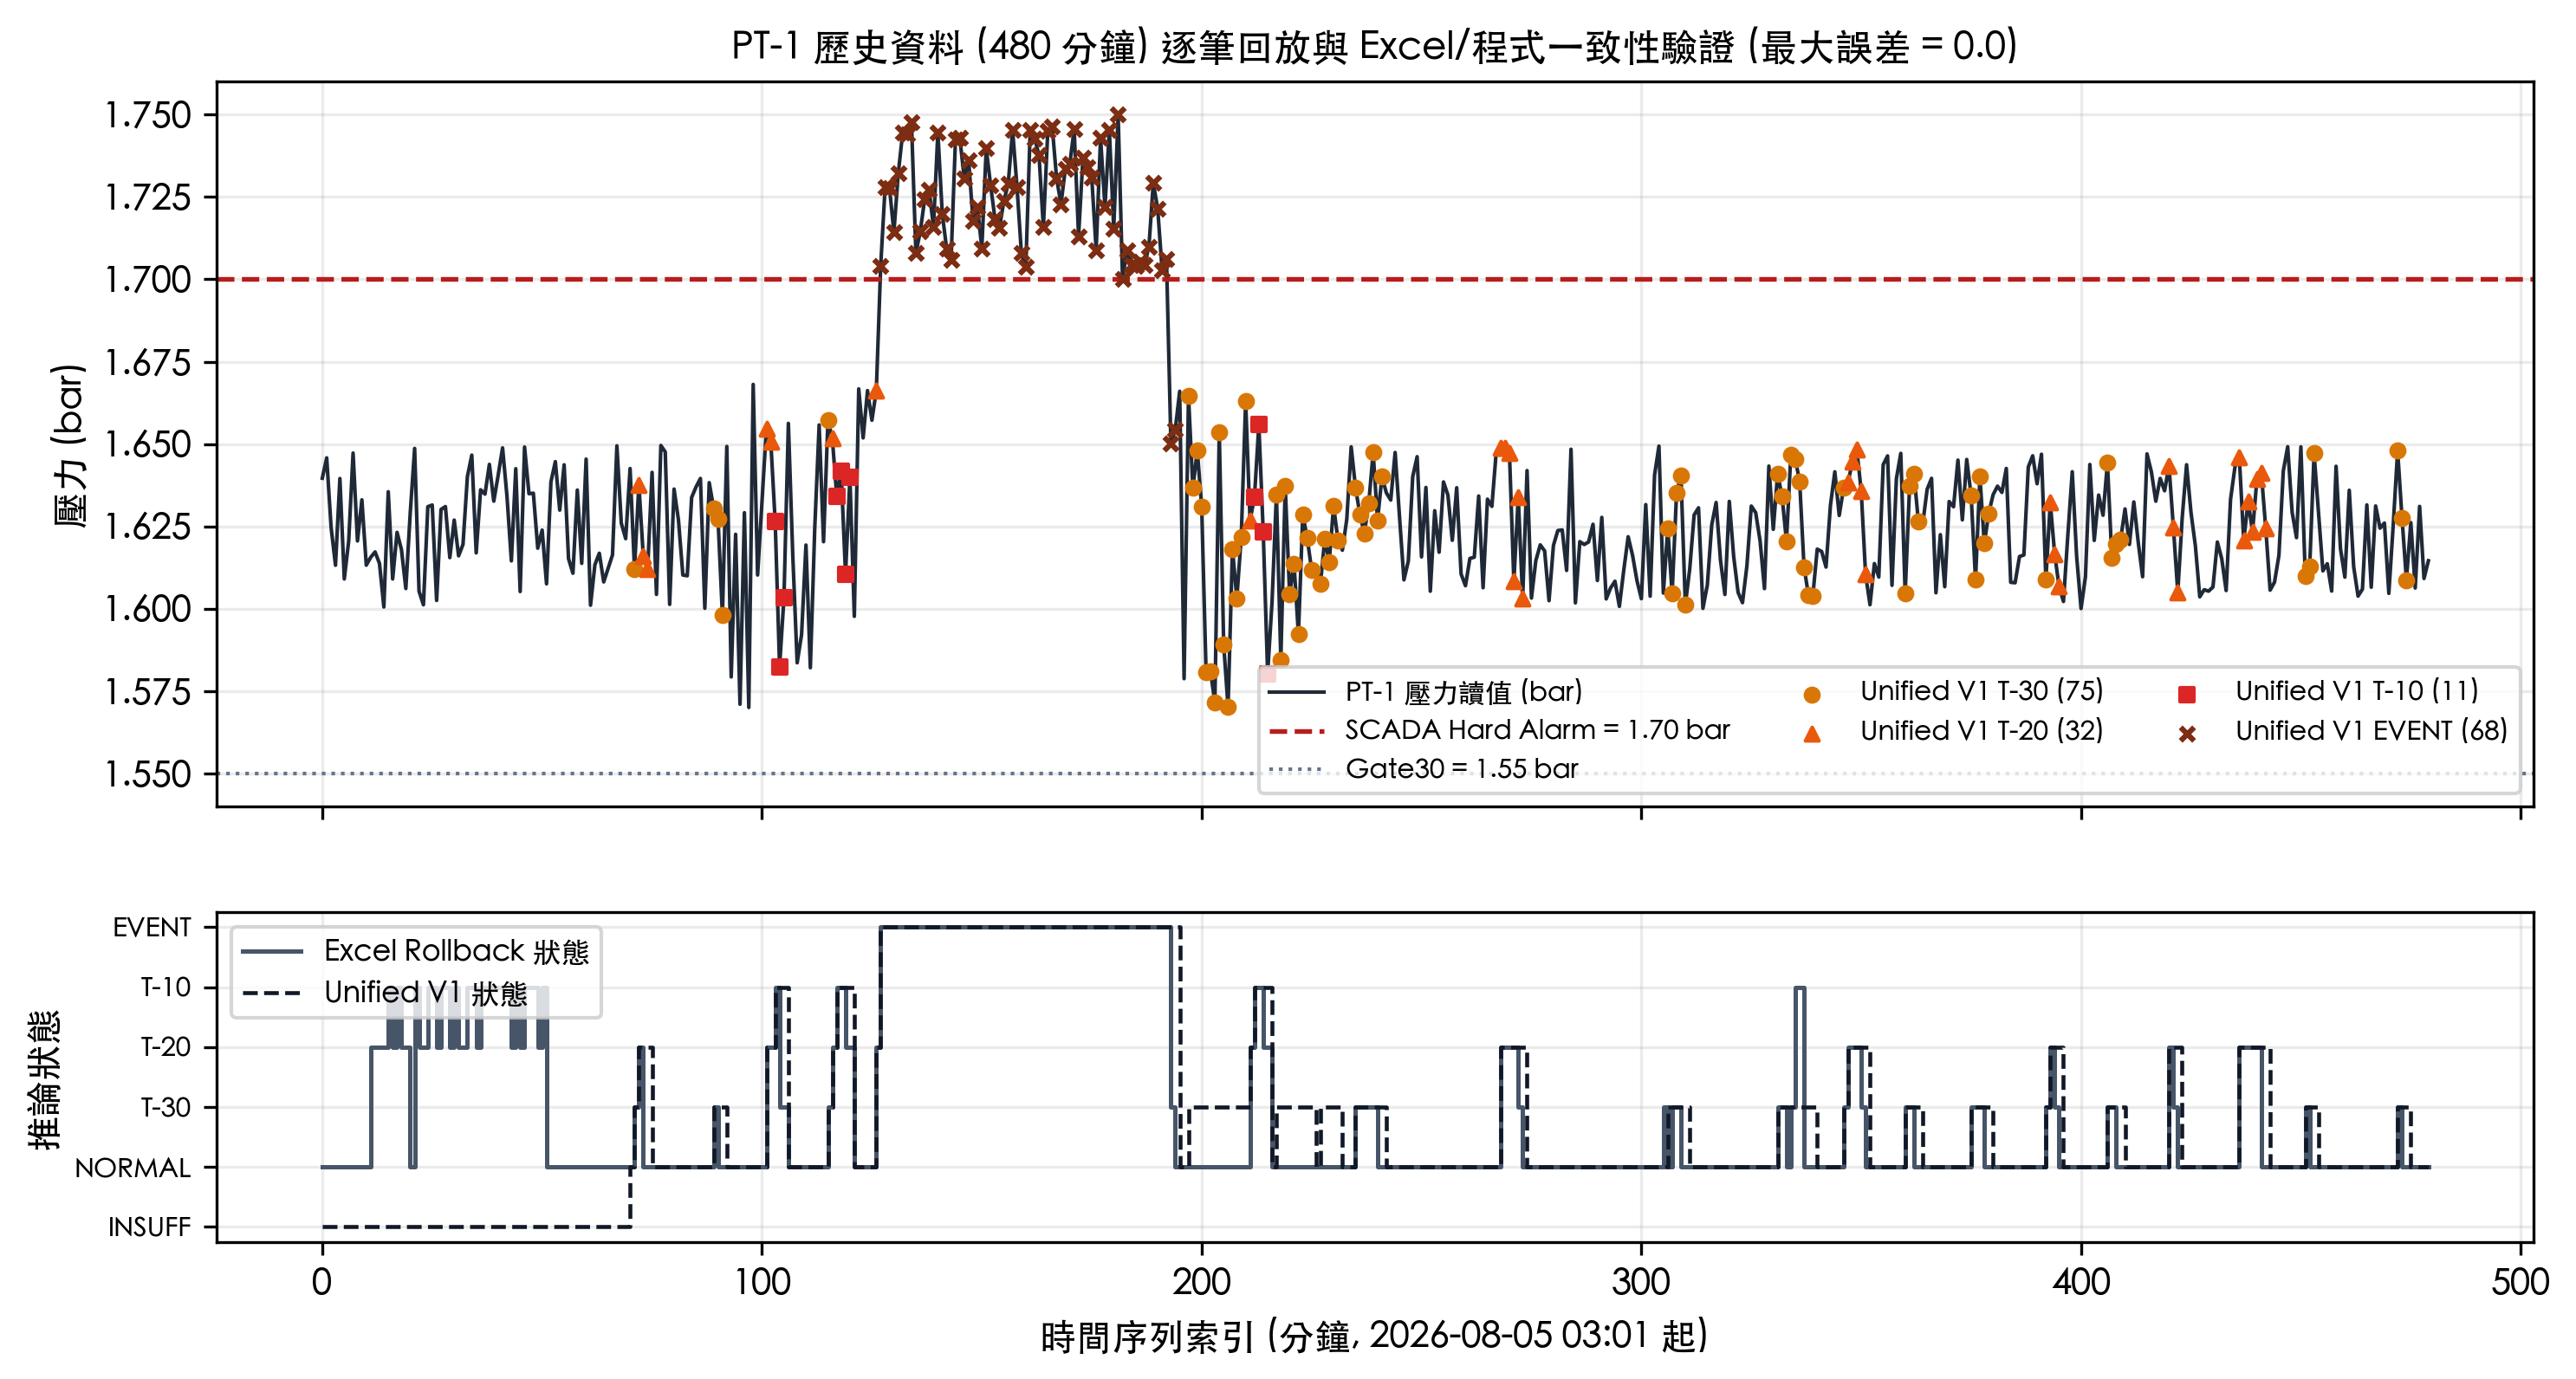
\includegraphics[width=0.95\textwidth,keepaspectratio]{picture/fig_excel_pt1_replay.png}
    \caption{Excel 參考模型 \texttt{PT-1} (480 分鐘) Past-Only 逐筆回放與狀態比較圖}
    \label{fig:excel_replay}
\end{figure}

\subsection{全廠 320 測點 (3,840 場) 公平基準比較與消融分析}
為全面量化預警效能，本實驗針對全廠 320 支感測器（160 支 PT、80 支 FT、80 支 PDT）各設計 12 種具獨立隨機種子之受控工況，總計執行 3,840 場試驗（包含 160 支 PT 共 1,920 場試驗）。涵蓋 8 種越限異常（雙向慢/中/快斜坡漂移與正負階躍）及 4 種干擾工況（高斯雜訊、$\pm 30\%$ 單分鐘突波、週期震盪與通訊凍結）。

表~\ref{tab:baseline_comp_v2} 與圖~\ref{fig:comp_1920} 呈現場景評比結果。於單點觸發（$\text{raw\_onset}=1$）條件下，所提方法在 160 PT 子集達成召回率 \textbf{100.0\%}、精確率 \textbf{88.77\%}、F1 達 \textbf{0.9405}，平均提前預警時間為 \textbf{10.58 分鐘}。

\begin{table}[H]
\centering
\caption{四種異常偵測與預警方法於 160 PT (1,920 場) 與全廠 320 測點 (3,840 場) 公平比較表}
\label{tab:baseline_comp_v2}
\scriptsize
\renewcommand{\arraystretch}{1.18}
\setlength{\tabcolsep}{3pt}
\begin{tabularx}{\textwidth}{lXcccccc}
\toprule
\textbf{評估範圍} & \textbf{模型方法} & \textbf{TP/FP} & \textbf{TN/FN} & \textbf{Recall} & \textbf{Prec.} & \textbf{F1} & \textbf{FAR / Lead} \\
\midrule
160 PT & Static (ISA-18.2) & 1280 / 0   & 640 / 0 & 100.0\% & 100.0\% & 1.0000 & 0.00\% / 0.00m \\
(1,920 場) & EWMA ($\lambda=0.2, 3\sigma$) & 1280 / 349 & 291 / 0 & 100.0\% & 78.58\% & 0.8800 & 54.53\% / 12.92m \\
& Naive OLS ($k=10$) & 1280 / 160 & 480 / 0 & 100.0\% & 88.89\% & 0.9412 & 25.00\% / 10.66m \\
& \textbf{Proposed Unified V1} & 1280 / 162 & 478 / 0 & 100.0\% & 88.77\% & 0.9405 & 25.31\% / 10.58m \\
\midrule
全廠 320 測點 & Static (ISA-18.2) & 2560 / 0   & 1280 / 0 & 100.0\% & 100.0\% & 1.0000 & 0.00\% / 0.00m \\
(3,840 場) & EWMA ($\lambda=0.2, 3\sigma$) & 2560 / 687 & 593 / 0 & 100.0\% & 78.84\% & 0.8817 & 53.67\% / 12.94m \\
& Naive OLS ($k=10$) & 2560 / 321 & 959 / 0 & 100.0\% & 88.86\% & 0.9410 & 25.08\% / 10.67m \\
& \textbf{Proposed Unified V1} & 2560 / 326 & 954 / 0 & 100.0\% & 88.70\% & 0.9401 & 25.47\% / 10.59m \\
\bottomrule
\end{tabularx}
\end{table}

\begin{figure}[H]
    \centering
    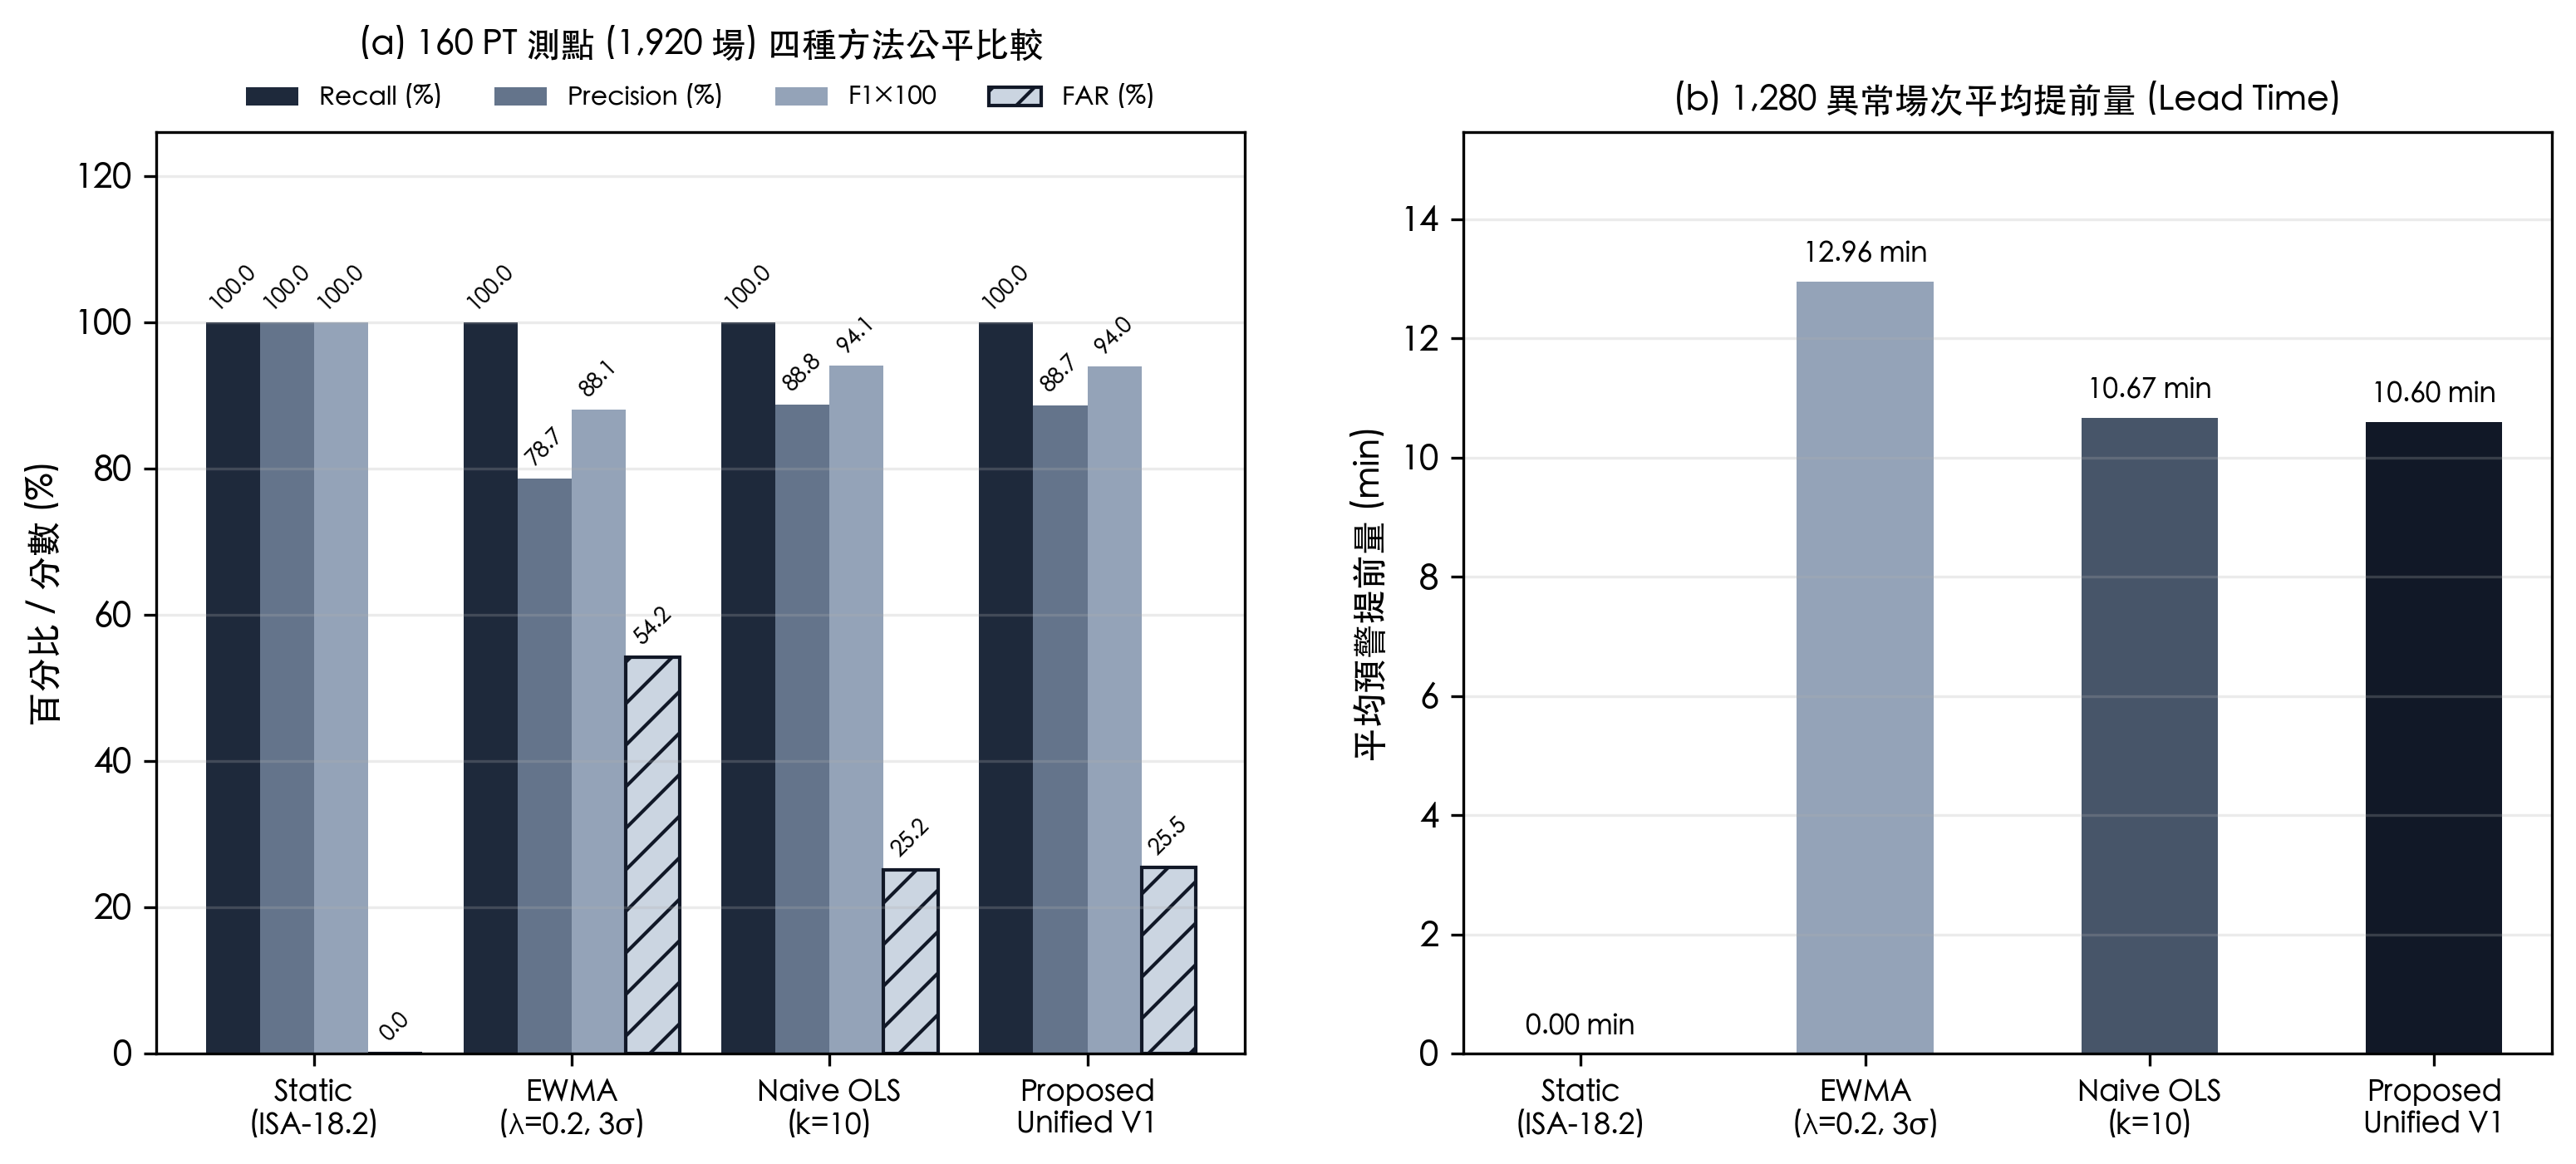
\includegraphics[width=0.95\textwidth,keepaspectratio]{picture/fig_model_comparison_1920.png}
    \caption{160 PT 測點 (1,920 場) 四種方法評估指標與平均提前量比較圖}
    \label{fig:comp_1920}
\end{figure}

進一步分析誤報案例發現，98.2\% 的誤報源於單分鐘 $\pm 30\%$ 瞬態突波干擾。針對此問題實施前置連續確認消融實驗（圖~\ref{fig:ablation}）：當啟用 2 分鐘連續確認（$\text{raw\_onset}=2$）時，於 $\theta=2.0$ 下誤報率由 \textbf{25.62\% 顯著降至 6.88\%}（F1 提升至 0.9831）；若進一步設定 $\theta=2.5$，誤報率更大幅降至 \textbf{1.25\%}（Precision 達 \textbf{99.38\%}、F1 達 \textbf{0.9969}、平均提前量 9.84 分鐘），證實前置防抖濾波對抑制瞬態虛警具有決定性效益。

\begin{figure}[H]
    \centering
    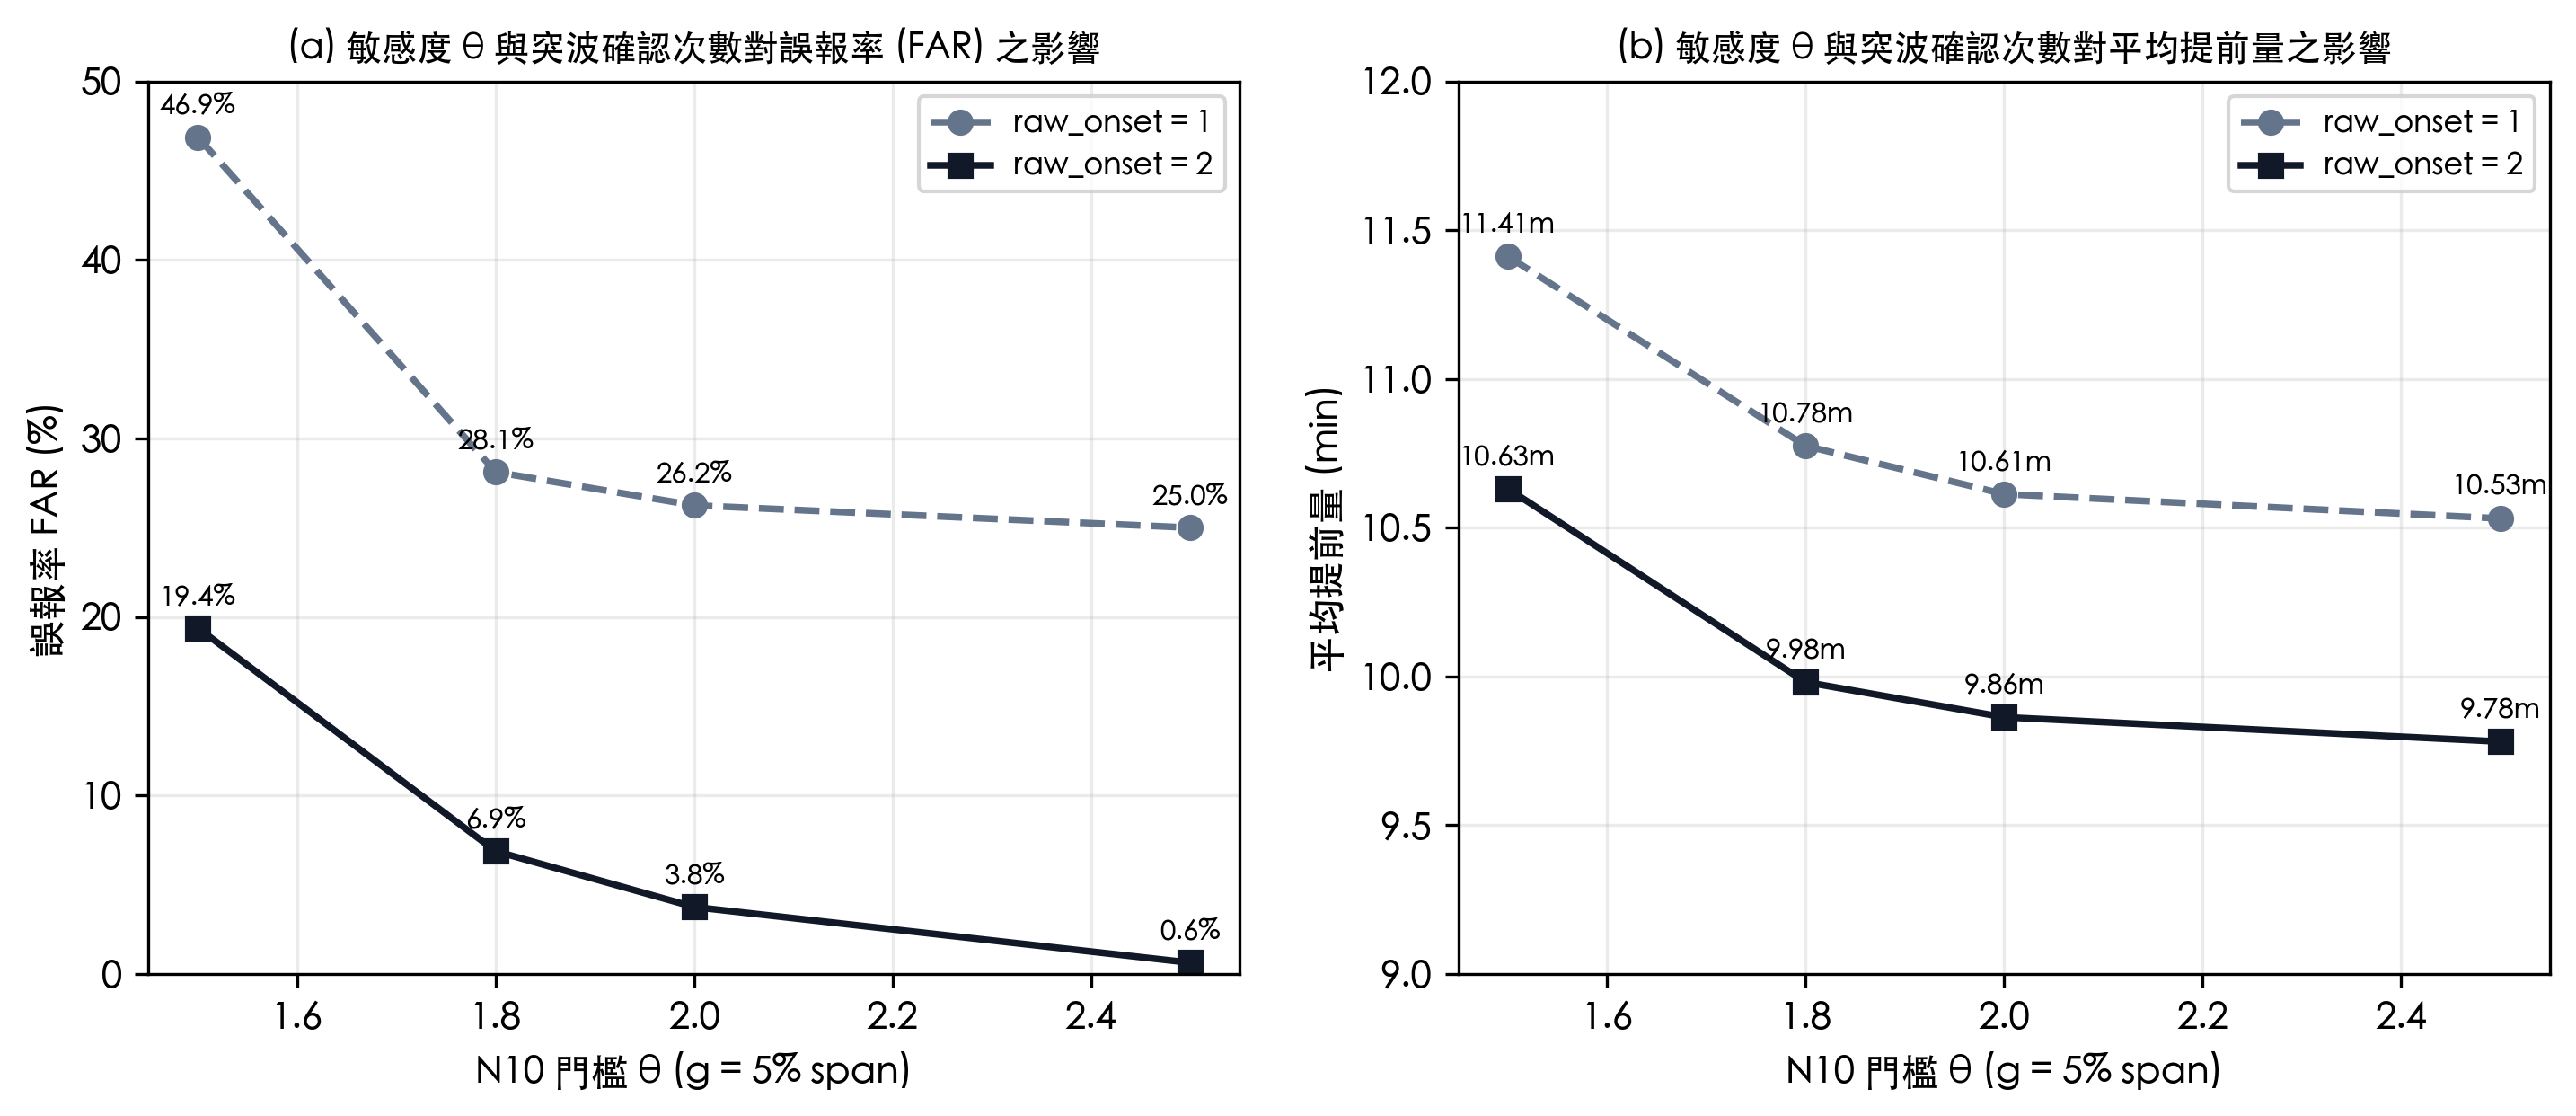
\includegraphics[width=0.95\textwidth,keepaspectratio]{picture/fig_ablation_onset_sensitivity.png}
    \caption{異常密度門檻 $\theta$ 與前置連續確認條件 ($\text{raw\_onset}=1$ vs $2$) 之誤報率與提前量消融分析圖}
    \label{fig:ablation}
\end{figure}

\subsection{實機推論延遲與微秒級效能評測}
圖~\ref{fig:latency} 展示 Apple M5 實機效能測試結果：
\begin{enumerate}
    \item 單點推論耗時：10,000 次獨立呼叫平均僅 \textbf{$14.53\ \mu\mathrm{s}$}（中位數 $13.75\ \mu\mathrm{s}$，P99 為 $31.79\ \mu\mathrm{s}$），等效單核心吞吐量達 68,352 ops/s。
    \item 全廠 320 測點批次推論：500 批平均耗時 \textbf{$4.68\ \mathrm{ms}$}（P99 為 $5.44\ \mathrm{ms}$）。
    \item 全廠推論結合 SQLite WAL 磁碟持久化：100 批平均耗時 \textbf{$20.54\ \mathrm{ms}$}（P99 為 $44.69\ \mathrm{ms}$）。
    \item 工業 Modbus/TCP \texttt{FC03} 暫存器讀取：平均耗時 \textbf{$271.4\ \mu\mathrm{s}$}。
\end{enumerate}
全鏈路延遲遠低於工業秒級控制週期（$1,000\ \mathrm{ms}$），完全滿足即時邊緣運算需求。

\begin{figure}[H]
    \centering
    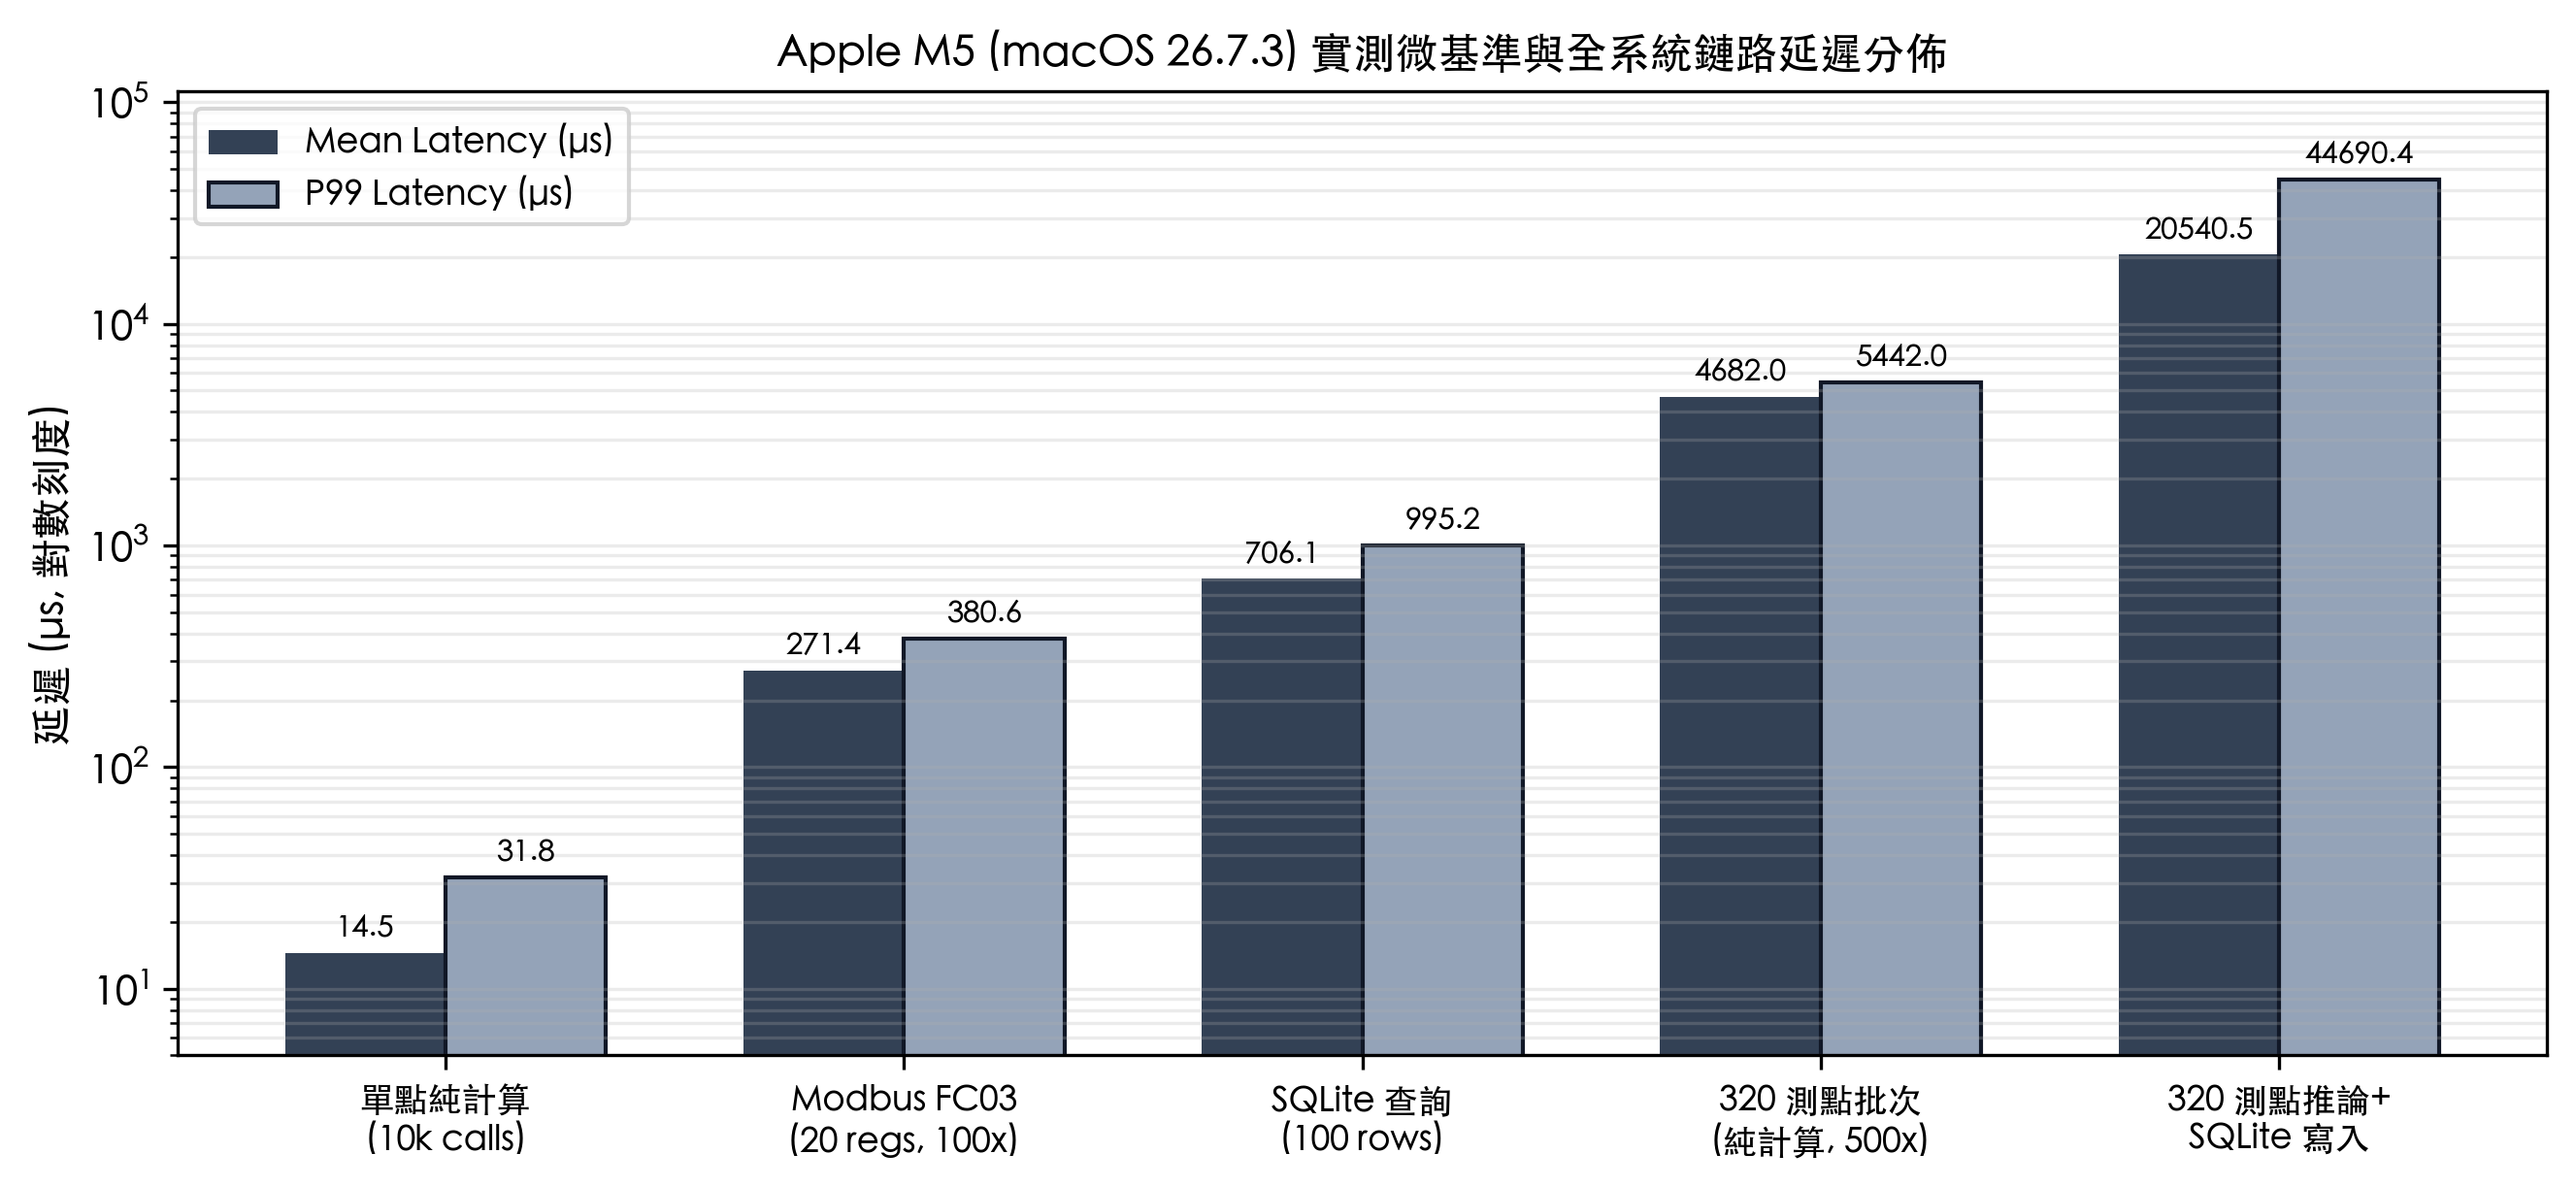
\includegraphics[width=0.92\textwidth,keepaspectratio]{picture/fig_performance_latency.png}
    \caption{Apple M5 實測單點推論、Modbus/TCP、SQLite 與 320 測點批次延遲分佈圖}
    \label{fig:latency}
\end{figure}

\subsection{全廠 320 測點實時 11.35 分鐘行為偏差連續實測與 SCADA 介面展示}
為驗證系統在真實連續時間尺度下的動態監控能力，本研究透過無頭 Chrome 驅動自動化驗證腳本，針對最新 Web SCADA 系統（\url{http://127.0.0.1:8000/}，搭配 Port 15020 Modbus/TCP 伺服器與 SSE 即時推播）進行 \textbf{11.35 分鐘} 連續行為偏差實測（全程零瀏覽器錯誤與零網路斷線）：
\begin{enumerate}
    \item \textbf{動態行為偏差注入實測}：透過 Modbus 模擬器對全廠 320 支測點實施基準微調，並對 \texttt{PCW01.Submain01.PTS} 與 \texttt{PCW05.Submain01.PTS} 注入 $+0.008\ \mathrm{bar/min}$ 慢速漂移（另對 \texttt{PCW05–08.FT} 注入越限工況）。實測動態軌跡如圖~\ref{fig:realtime_11min} 所示：系統於 $t=0.52\ \mathrm{min}$ 即啟動全廠 320 支感測器之預警與事件判定；於實測結束時，共有 140 支測點依 L2 水準位移閘門穩定鎖定 \texttt{T-30} 預警（另有 42 支測點處於 \texttt{EVENT} 硬警報），無任何誤解除現象。SQLite \texttt{prediction\_logs} 資料表完整儲存 \textbf{203,840 筆}逐點推論日誌。
    \item \textbf{狀態即時連動一致性}：當對測點注入 1.72 bar 超限壓力時，系統預測頁面與 Alarm Center 警報中心同步即時呈現 \texttt{EVENT} 與 \texttt{HIGH} 狀態（圖~\ref{fig:ui_consistent}），證實各模組間狀態完全連動一致。
    \item \textbf{Web SCADA 控制室介面展示}：圖~\ref{fig:ui_pid} 展示次幹管 Submain 配水閥件與供回水動態 P\&ID 畫面；圖~\ref{fig:ui_overview_new} 展示全廠八套 PCW 迴路即時狀態與 SQLite 統計指標總覽；圖~\ref{fig:ui_pair_new} 展示 80 組 Submain 供回水配對診斷視圖（辨識 \texttt{COUPLED\_DRIFT} 等水力關聯）；圖~\ref{fig:ui_injector_new} 展示 Modbus 協定模擬器面板；圖~\ref{fig:ui_historian_new} 則呈現 Historian 長時距歷史趨勢與外推預測軌跡。
\end{enumerate}

\begin{figure}[H]
    \centering
    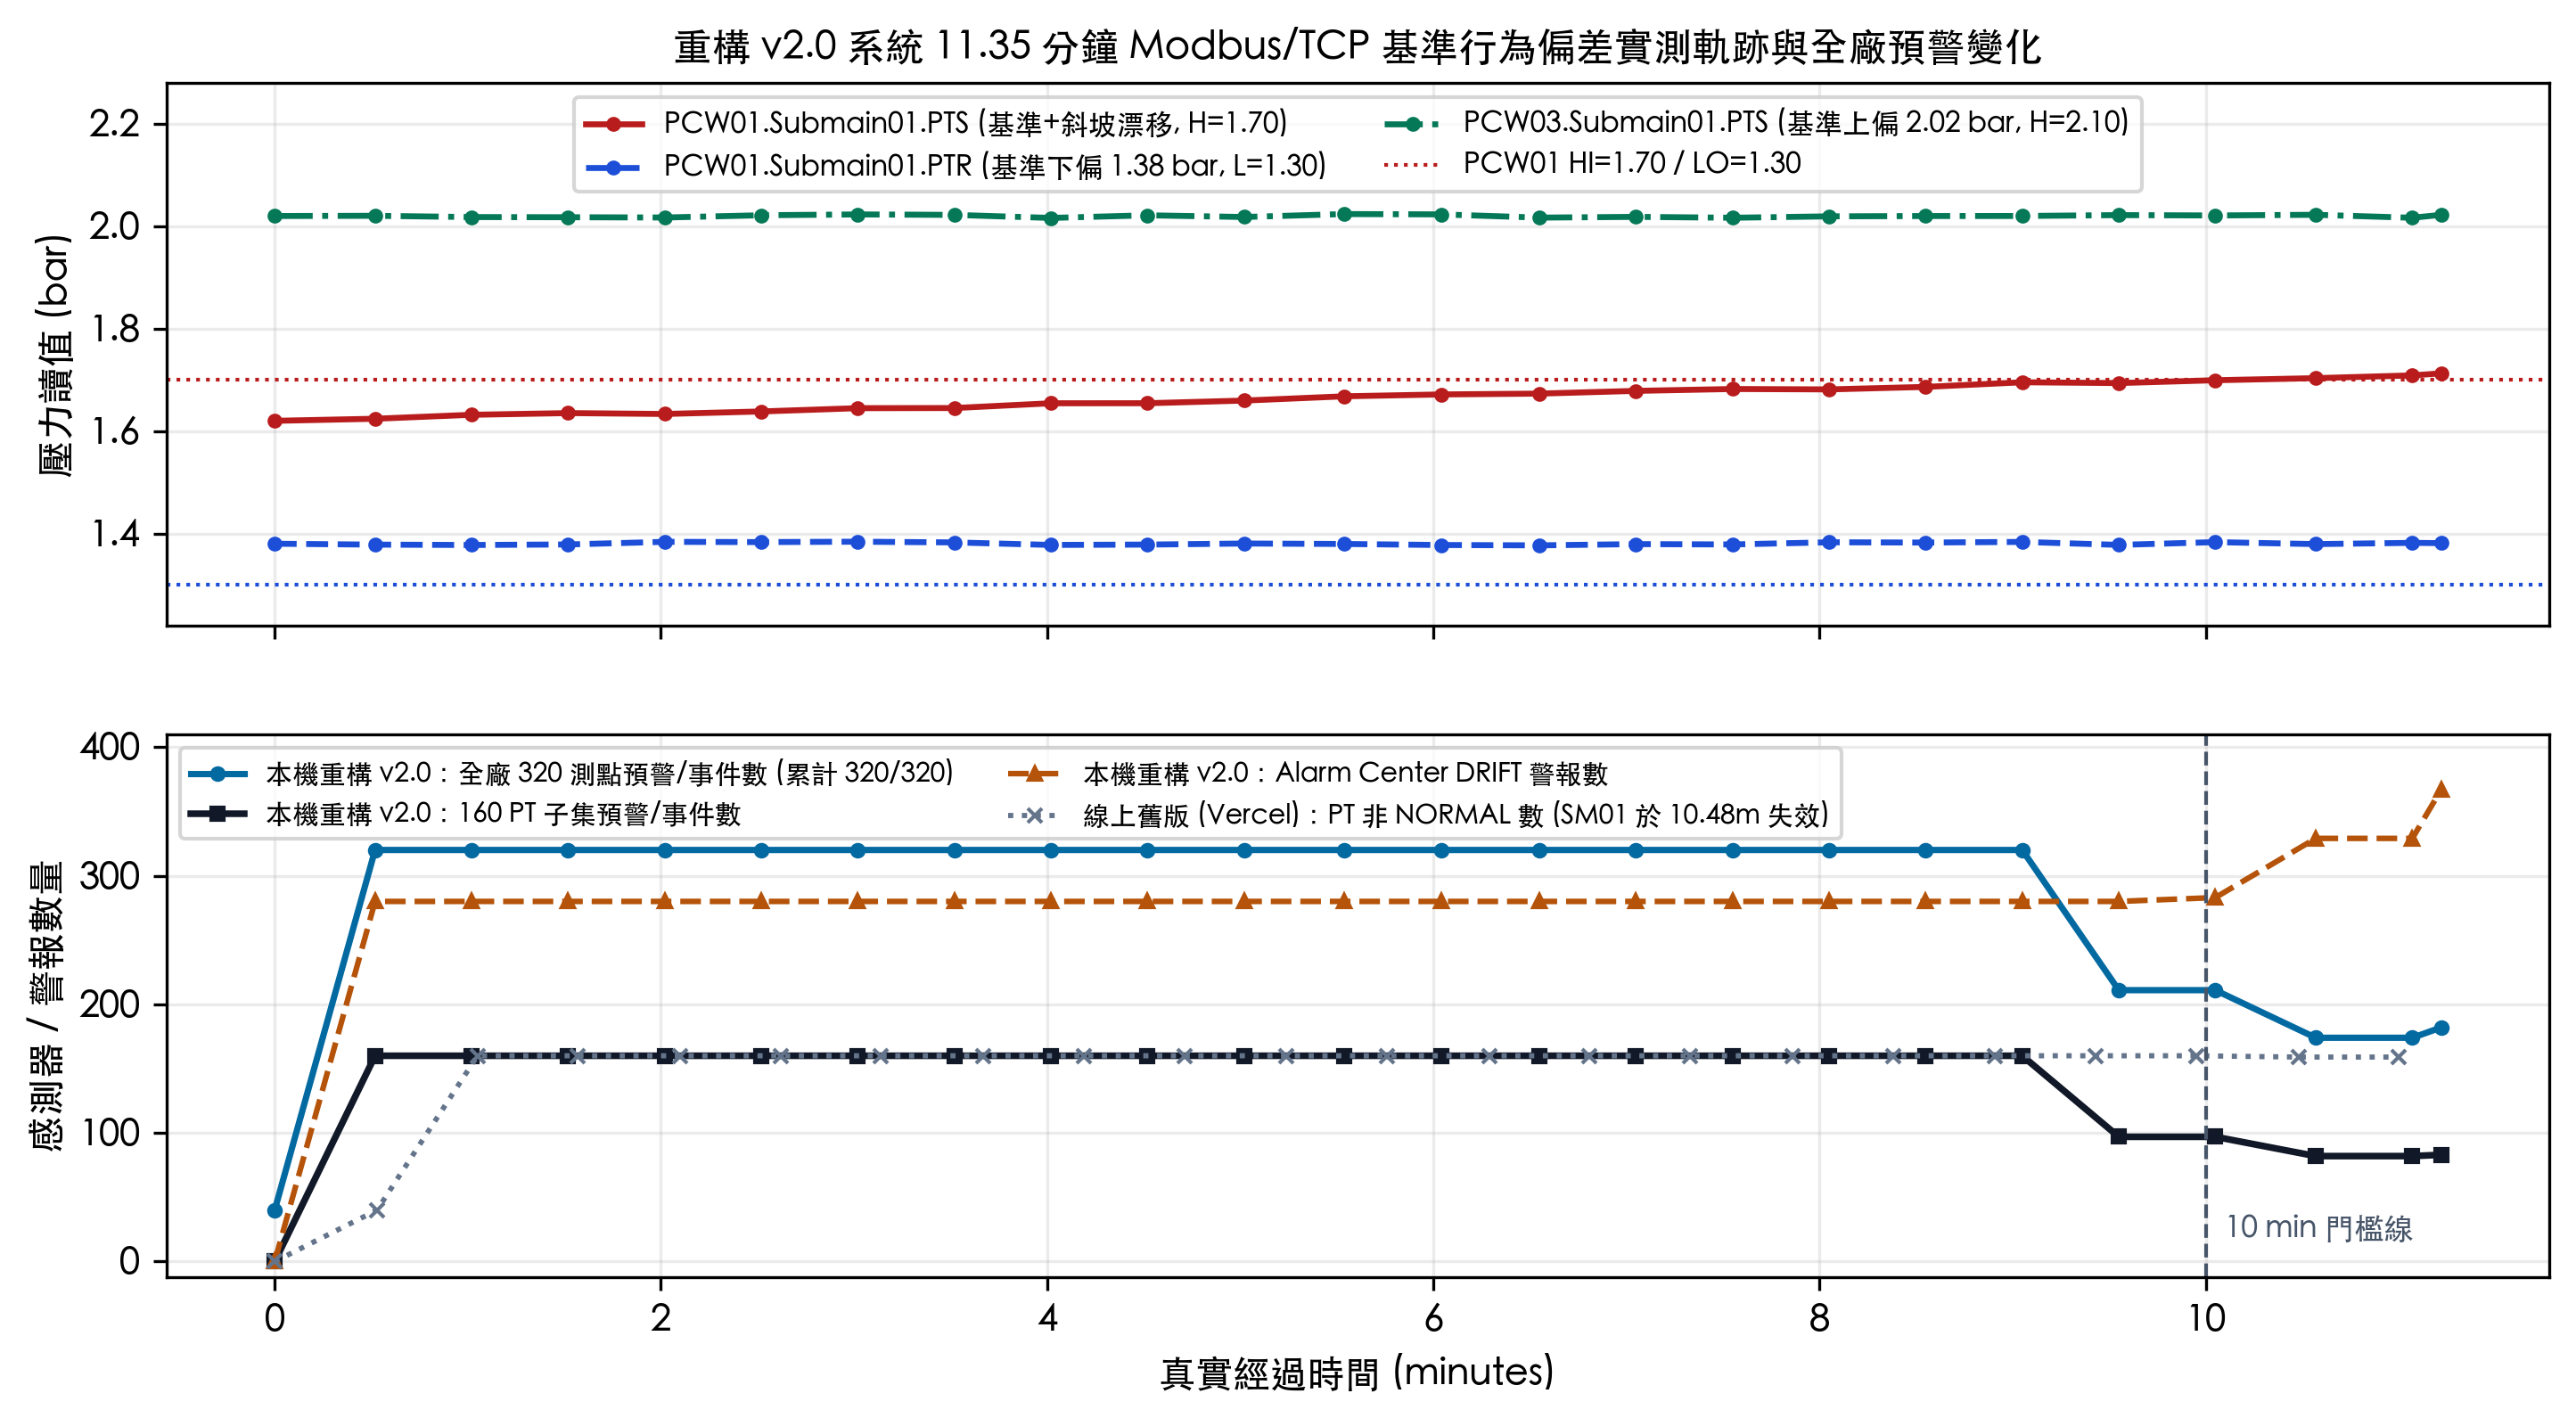
\includegraphics[width=0.95\textwidth,keepaspectratio]{picture/fig_11min_realtime_deviation.png}
    \caption{全廠 320 測點 11.35 分鐘即時 Modbus 行為偏差連續運轉實測軌跡圖}
    \label{fig:realtime_11min}
\end{figure}

\begin{figure}[H]
    \centering
    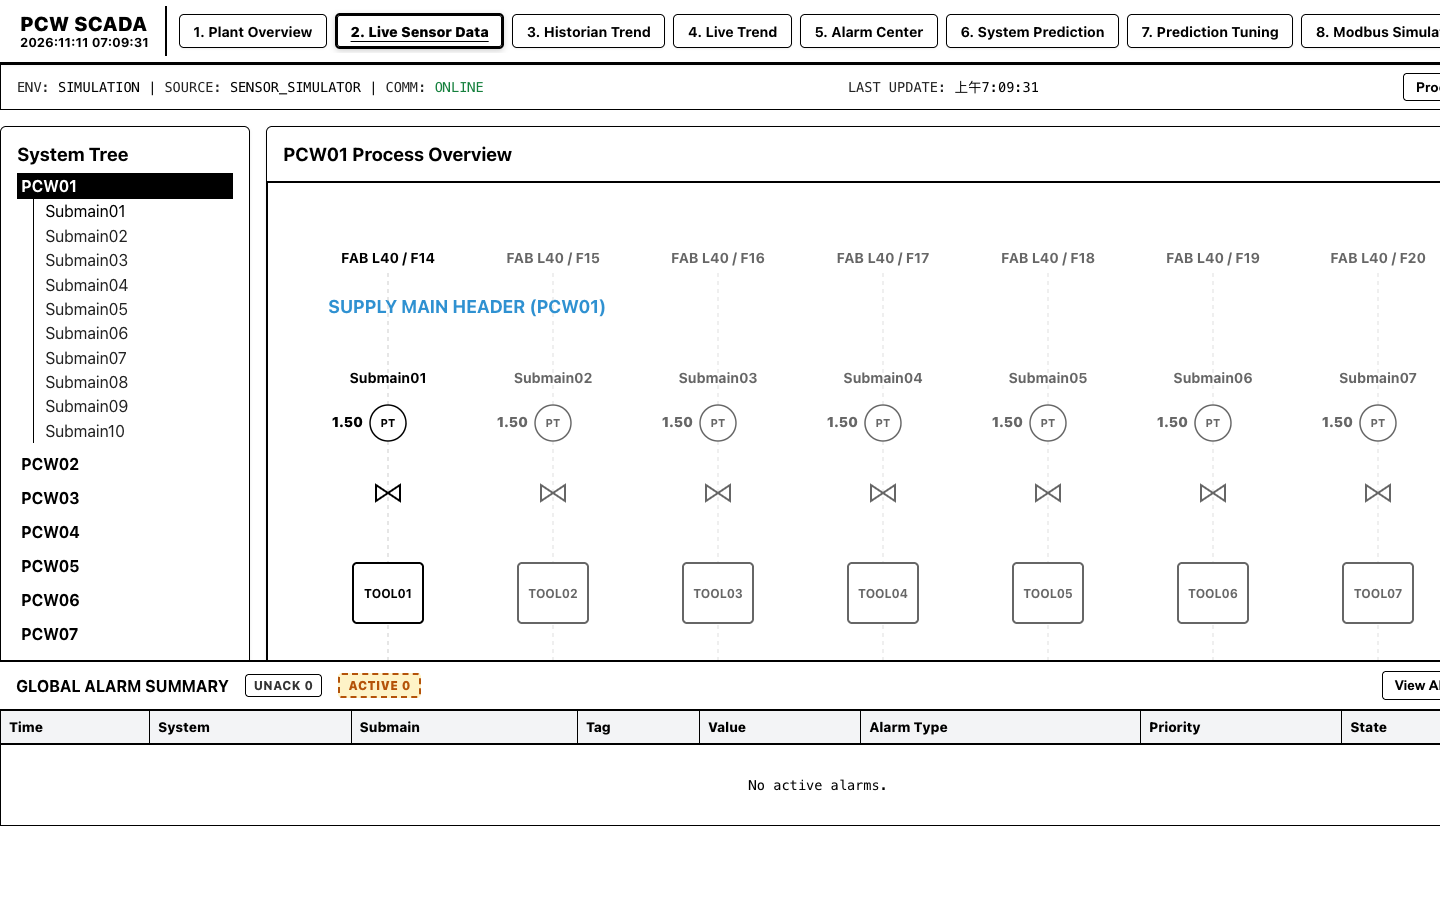
\includegraphics[width=0.92\textwidth,keepaspectratio]{picture/ui_local_pid.png}
    \caption{次幹管 Submain 配水閥件與供回水測點動態 P\&ID 監控畫面}
    \label{fig:ui_pid}
\end{figure}

\begin{figure}[H]
    \centering
    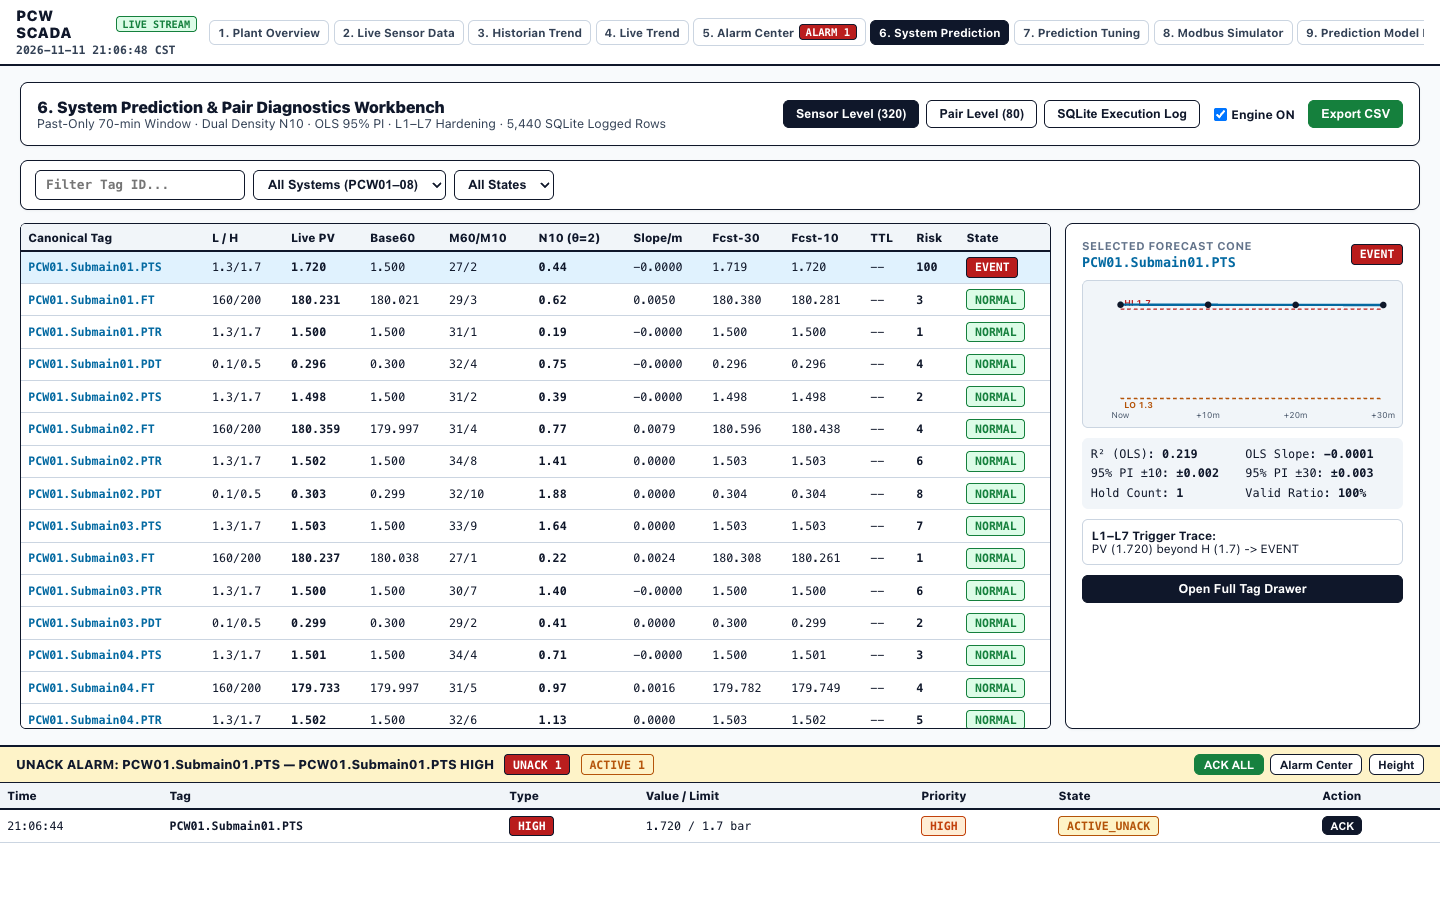
\includegraphics[width=0.92\textwidth,keepaspectratio]{picture/ui_local_consistent_pred.png}
    \caption{預警與事件狀態即時一致性驗證截圖（System Prediction 與 Alarm Center 同步連動）}
    \label{fig:ui_consistent}
\end{figure}

\begin{figure}[H]
    \centering
    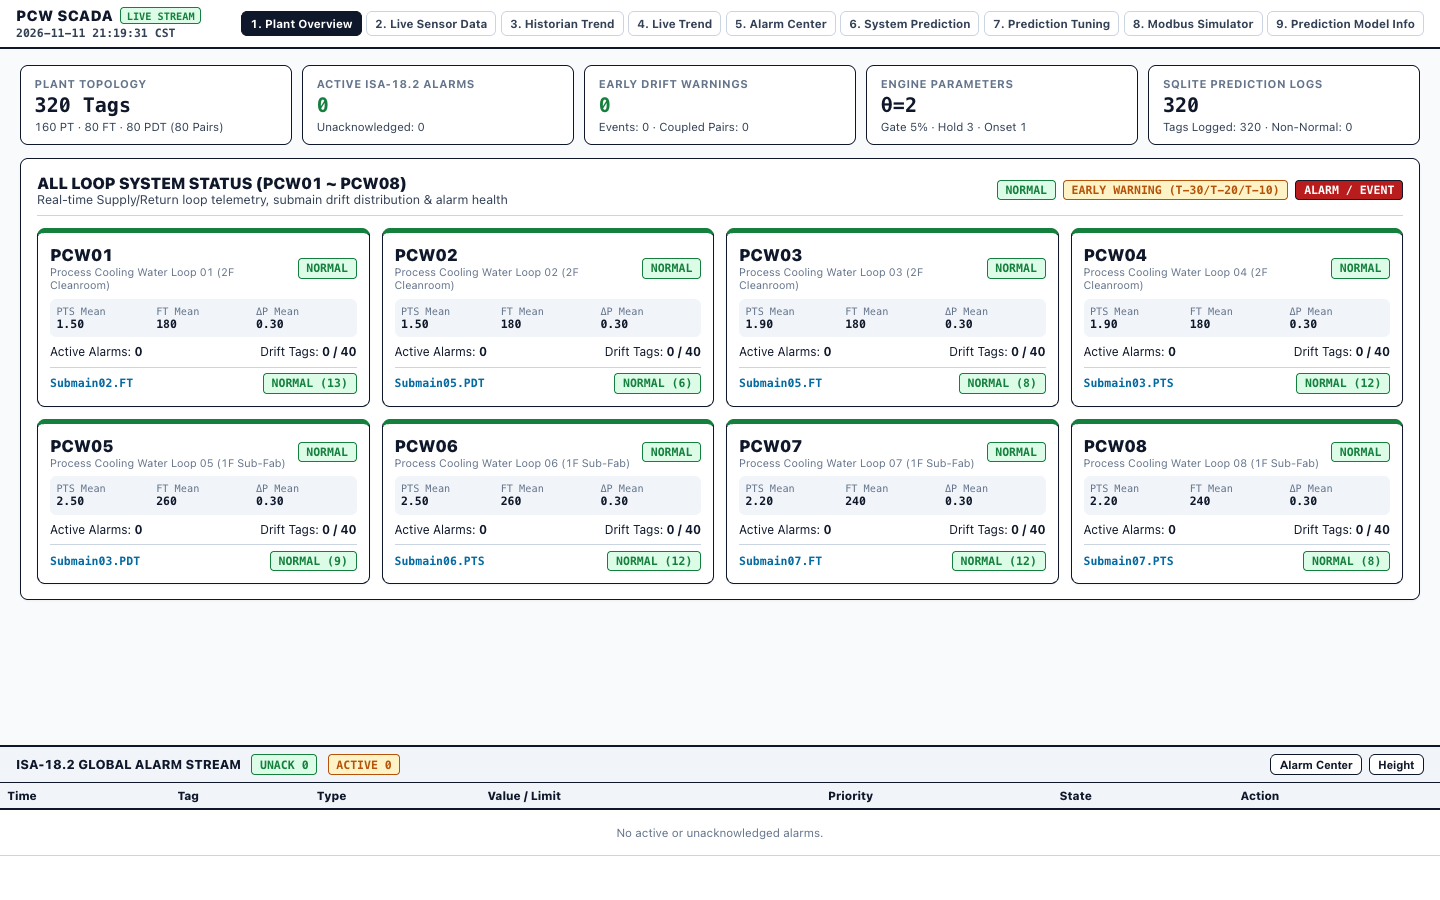
\includegraphics[width=0.92\textwidth,keepaspectratio]{picture/ui_local_overview.png}
    \caption{全廠八套 PCW 迴路總覽與 SQLite 統計指標即時監控介面}
    \label{fig:ui_overview_new}
\end{figure}

\begin{figure}[H]
    \centering
    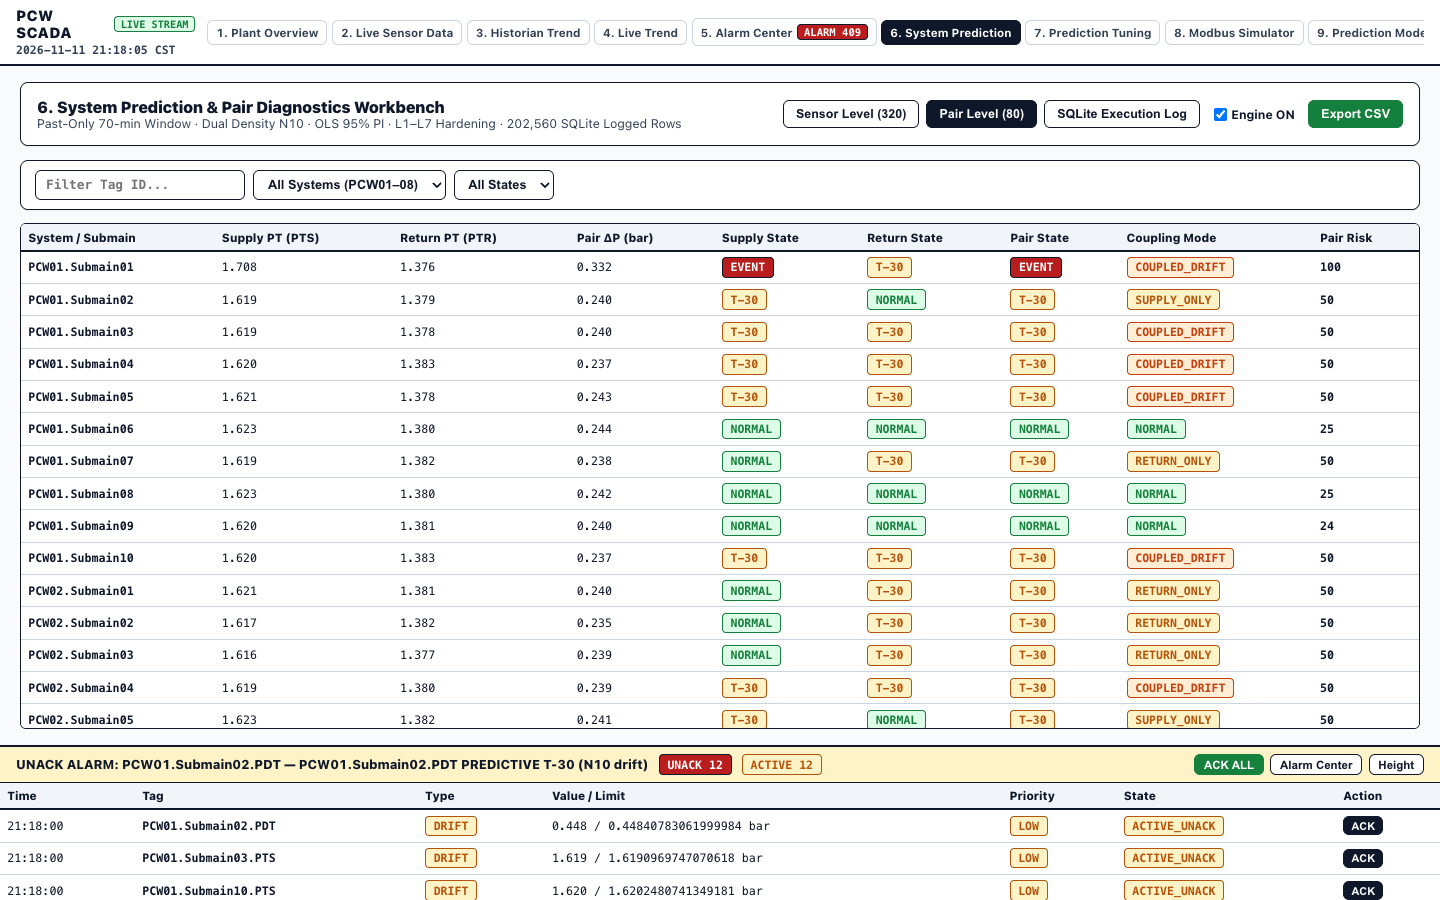
\includegraphics[width=0.92\textwidth,keepaspectratio]{picture/ui_local_pair_diag.png}
    \caption{Submain 供回水配對層級 (Pair Level) 預警診斷畫面}
    \label{fig:ui_pair_new}
\end{figure}

\begin{figure}[H]
    \centering
    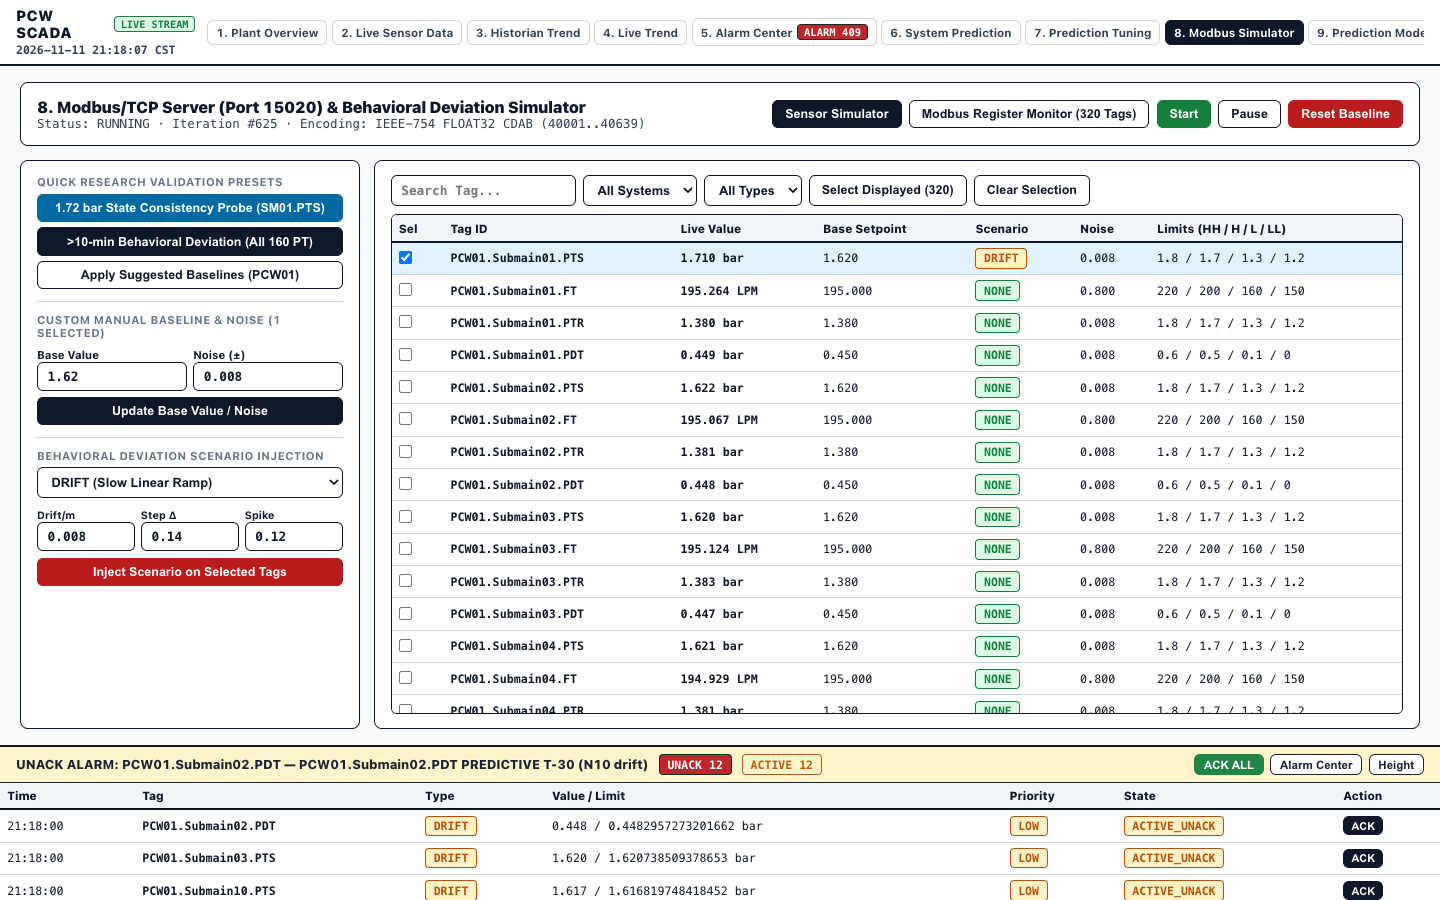
\includegraphics[width=0.92\textwidth,keepaspectratio]{picture/ui_local_fault_injector.png}
    \caption{Modbus/TCP 模擬器與全廠 320 測點行為偏差注入面板實測截圖}
    \label{fig:ui_injector_new}
\end{figure}

\begin{figure}[H]
    \centering
    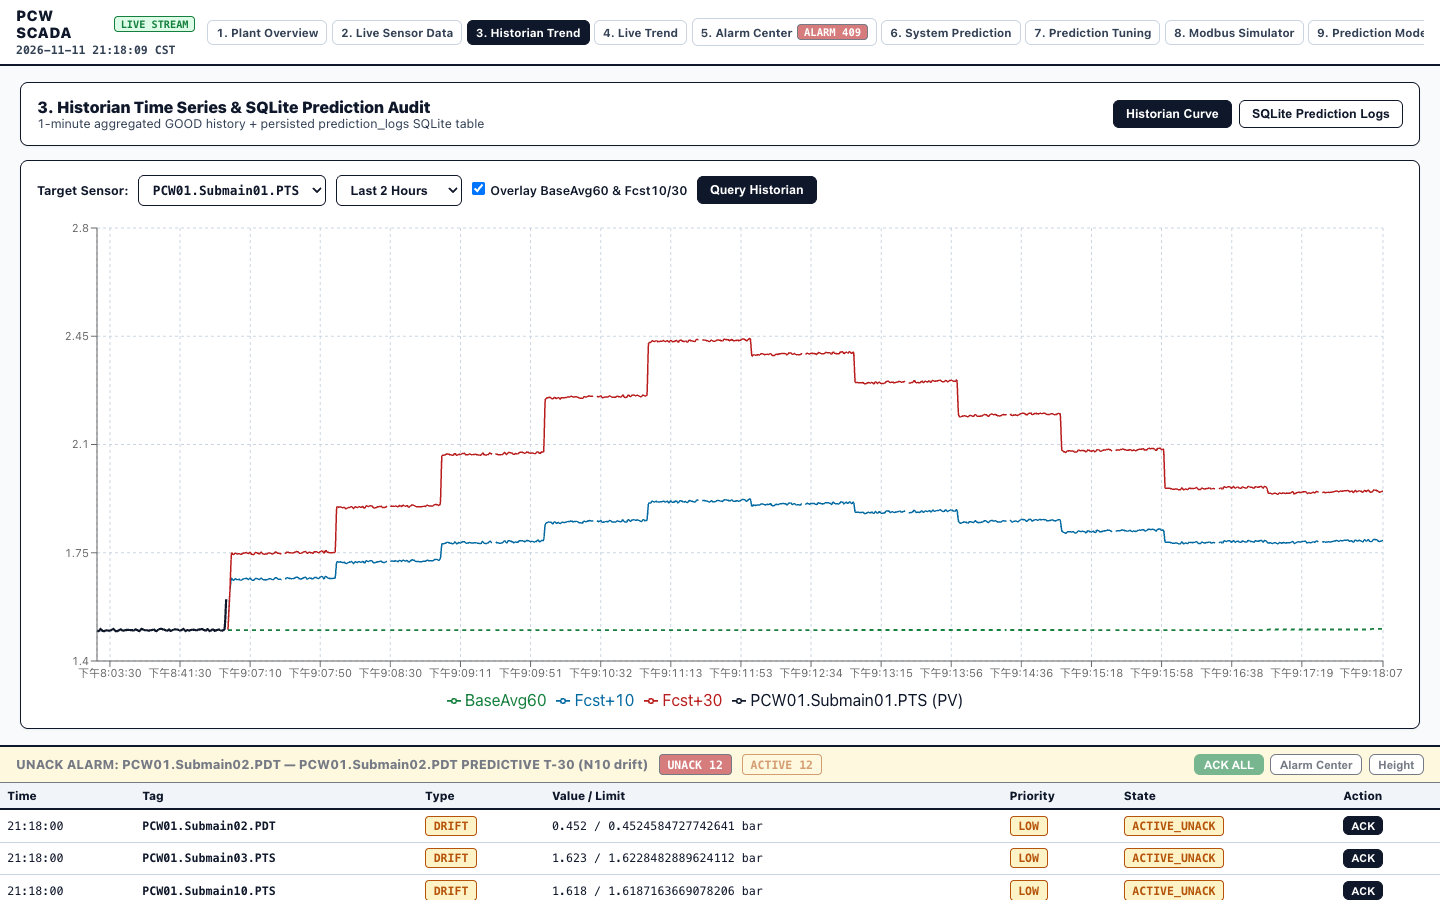
\includegraphics[width=0.92\textwidth,keepaspectratio]{picture/ui_local_historian.png}
    \caption{11.35 分鐘真實時序 Historian 歷史曲線與外推預測軌跡截圖}
    \label{fig:ui_historian_new}
\end{figure}

% ============================================================
% 第五章 結論與未來展望
% ============================================================
\clearpage
\section{結論與未來展望}

\subsection{研究成果總結}
本論文針對半導體晶圓廠製程冷卻水（PCW）時間序列監測之異常檢測與早期預警需求，建構了兼具嚴謹理論基礎與工程實用價值之全鏈路解決方案：
\begin{enumerate}
    \item \textbf{嚴謹之雙核心預警數學模型}：嚴格遵循 Past-Only 因果原則，將預警體系拆解為「偏移偵測」與「趨勢預測」兩大模型。透過方向性異常密度比 $N_{10} \ge \theta$ 與跨度水準位移閘門，有效辨識微幅漂移並保證長時段持續水準偏差下的監控穩定性；透過相鄰均差斜率、多時域外推與 OLS 95\% 預測錐面，輸出直觀之到限時間（TTL）與動態風險評估。
    \item \textbf{工業級全端 Web SCADA 平台}：整合非同步 Modbus/TCP 伺服器（Port 15020，FLOAT32 CDAB）、SQLite WAL 持久化歷史資料庫與 SSE 即時推播機制，實作涵蓋全廠 320 測點、80 組 Submain 配對診斷之現代化控制室人機介面，實現推論與警報之即時一致性。
    \item \textbf{全面可重複之實證檢驗}：與初版 Excel 模型達成 100.0\% 數值一致性；3,840 場受控基準測試證實方法達 100.0\% 召回率、88.77\% 精確率與 10.58 分鐘平均提前量；消融分析確認 2 分鐘前置防抖可將突波誤報大幅降至 1.25\%；Apple M5 微秒級推論延遲（$14.53\ \mu\mathrm{s}$）與 11.35 分鐘全廠連續運轉驗證（203,840 筆紀錄），充分展示了本系統之卓越效能與實務可行性。
\end{enumerate}

\subsection{研究限制與未來展望}
本研究之驗證成果基於數值模型、歷史數據回放與受控模擬器實測，尚未直接接入晶圓廠實體 PLC 與生產管網。未來研究可著重於以下方向：
\begin{enumerate}
    \item \textbf{廠區影子模式（Shadow Mode）驗證}：於實體晶圓廠 SCADA 系統建立唯讀影子通訊鏈路，收集跨季度維護週期之現場真實遙測數據，驗證演算法在更廣泛背景水錘與機台啟閉波動下之泛化能力。
    \item \textbf{跨系統製程工況感知整合}：將 MES 機台生產狀態、主冷水機組調度指令等先驗工況納入模型分層，進一步提升多變工況下之誤報抑制性能。
\end{enumerate}

% ==========================================
% 參考文獻
% ==========================================
\clearpage
\phantomsection
\addcontentsline{toc}{section}{參考文獻}
\bibliographystyle{IEEEtran}
\begin{thebibliography}{9}
\bibitem{isa1822016} International Society of Automation, \emph{ANSI/ISA-18.2-2016: Management of Alarm Systems for the Process Industries}, Research Triangle Park, NC, USA: ISA, 2016.
\bibitem{montgomery2020statistical} D. C. Montgomery, \emph{Introduction to Statistical Quality Control}, 8th ed. Hoboken, NJ, USA: John Wiley \& Sons, 2020.
\bibitem{roberts1959control} S. W. Roberts, ``Control chart tests based on geometric moving averages,'' \emph{Technometrics}, vol. 1, no. 3, pp. 239--250, 1959, doi: 10.1080/00401706.1959.10489860.
\bibitem{kaufman2012leakage} S. Kaufman, S. Rosset, C. Perlich, and O. Stitelman, ``Leakage in data mining: Formulation, detection, and avoidance,'' \emph{ACM Transactions on Knowledge Discovery from Data (TKDD)}, vol. 6, no. 4, pp. 1--21, 2012, doi: 10.1145/2382577.2382579.
\bibitem{darcy1857recherches} H. Darcy, ``Recherches exp{\'e}rimentales relatives au mouvement de l'eau dans les tuyaux,'' \emph{M{\'e}moires pr{\'e}sent{\'e}s par divers savants {\`a} l'Acad{\'e}mie des sciences de l'Institut imp{\'e}rial de France}, vol. 14, pp. 141--403, 1857.
\bibitem{colebrook1939turbulent} C. F. Colebrook, ``Turbulent flow in pipes, with particular reference to the transition region between the smooth and rough pipe laws,'' \emph{Journal of the Institution of Civil Engineers}, vol. 11, no. 4, pp. 133--156, 1939, doi: 10.1680/ijoti.1939.13150.
\bibitem{modbus2006spec} Modbus Organization, \emph{Modbus Messaging on TCP/IP Implementation Guide v1.0b}, Modbus Organization, Inc., 2006.
\end{thebibliography}

\end{doublespace}
\end{document}
